%%%%%%%% ICML 2025 EXAMPLE LATEX SUBMISSION FILE MODIFIED FOR ARXIV %%%%%%%%%%%%%%%%%

\documentclass{article}

% Recommended, but optional, packages for figures and better typesetting:
\usepackage{microtype}
\usepackage{graphicx}
\usepackage{subfigure}
\usepackage{multirow}
\usepackage{enumitem}
\usepackage{booktabs} % for professional tables

% hyperref makes hyperlinks in the resulting PDF.
% If your build breaks (sometimes temporarily if a hyperlink spans a page)
% please comment out the following usepackage line and replace
% \usepackage{icml2025} with \usepackage[nohyperref]{icml2025} above.
\usepackage{hyperref}


% Attempt to make hyperref and algorithmic work together better:
\newcommand{\theHalgorithm}{\arabic{algorithm}}

% Use the following line for the initial ARXIV version
\usepackage[accepted]{icml2025arxiv}



% For theorems and such
\usepackage{amsmath}
\usepackage{amssymb}
\usepackage{mathtools}
\usepackage{amsthm}
\usepackage{bm}

% if you use cleveref..
\usepackage[capitalize,noabbrev]{cleveref}

%%%%%%%%%%%%%%%%%%%%%%%%%%%%%%%%
% THEOREMS
%%%%%%%%%%%%%%%%%%%%%%%%%%%%%%%%
\theoremstyle{plain}
\newtheorem{theorem}{Theorem}[section]
\newtheorem{proposition}[theorem]{Proposition}
\newtheorem{lemma}[theorem]{Lemma}
\newtheorem{corollary}[theorem]{Corollary}
\theoremstyle{definition}
\newtheorem{definition}[theorem]{Definition}
\newtheorem{assumption}[theorem]{Assumption}
\theoremstyle{remark}
\newtheorem{remark}[theorem]{Remark}
\newtheorem{example}[theorem]{Example}


\DeclareMathOperator*{\argmax}{arg\,max}
\DeclareMathOperator*{\argmin}{arg\,min}

\newcommand{\jannis}[1]{\textcolor{red}{ #1 }}
\newcommand{\ilker}[1]{\textcolor{blue}{ #1 }}


% Todonotes is useful during development; simply uncomment the next line
%    and comment out the line below the next line to turn off comments
%\usepackage[disable,textsize=tiny]{todonotes}
\usepackage[textsize=tiny]{todonotes}


% The \icmltitle you define below is probably too long as a header.
% Therefore, a short form for the running title is supplied here:
\icmltitlerunning{Coherent Local Explanations for Mathematical Optimization}

\usepackage{comment}

\begin{document}

\twocolumn[
\icmltitle{Coherent Local Explanations for Mathematical Optimization}


% It is OKAY to include author information, even for blind
% submissions: the style file will automatically remove it for you
% unless you've provided the [accepted] option to the icml2025
% package.

% List of affiliations: The first argument should be a (short)
% identifier you will use later to specify author affiliations
% Academic affiliations should list Department, University, City, Region, Country
% Industry affiliations should list Company, City, Region, Country

% You can specify symbols, otherwise they are numbered in order.
% Ideally, you should not use this facility. Affiliations will be numbered
% in order of appearance and this is the preferred way.
% \icmlsetsymbol{equal}{*}

\begin{icmlauthorlist}
\icmlauthor{Daan Otto}{yyy}
\icmlauthor{Jannis Kurtz}{yyy}
\icmlauthor{Ilker Birbil}{yyy}
\end{icmlauthorlist}

\icmlaffiliation{yyy}{Amsterdam Business School, University of Amsterdam, Amsterdam, The Netherlands}

\icmlcorrespondingauthor{Daan Otto}{d.otto@uva.nl}

% You may provide any keywords that you
% find helpful for describing your paper; these are used to populate
% the "keywords" metadata in the PDF but will not be shown in the document
\icmlkeywords{Machine Learning, ICML, Operations Research, Explainability}

\vskip
0.3in]

% this must go after the closing bracket ] following \twocolumn[ ...

% This command actually creates the footnote in the first column
% listing the affiliations and the copyright notice.
% The command takes one argument, which is text to display at the start of the footnote.
% The \icmlEqualContribution command is standard text for equal contribution.
% Remove it (just {}) if you do not need this facility.
\printAffiliationsAndNotice{}  % leave blank if no need to mention equal contribution
% \printAffiliationsAndNotice{\icmlEqualContribution} % otherwise use the standard text.

% \begin{abstract}
% The surge of explainable artificial intelligence methods seeks to enhance transparency and explainability in machine learning models. At the same time, there is a growing demand for explaining decisions taken through complex algorithms used in mathematical optimization.
% In response to this need, we introduce Coherent Local Explanations for Mathematical Optimization (CLEMO). CLEMO provides explanations for multiple components of optimization models, the objective value and decision variables, which are coherent with the underlying model structure. Our sampling-based procedure can provide explanations for the behavior of exact and heuristic solution algorithms. The effectiveness of CLEMO is illustrated by experiments for the shortest path problem, the knapsack problem, and the vehicle routing problem.
% \end{abstract}

\begin{abstract}
The surge of explainable artificial intelligence methods seeks to enhance transparency and explainability in machine learning models. At the same time, there is a growing demand for explaining decisions taken through complex algorithms used in mathematical optimization. However, current explanation methods do not take into account the structure of the underlying optimization problem, leading to unreliable outcomes. In response to this need, we introduce Coherent Local Explanations for Mathematical Optimization (CLEMO). CLEMO provides explanations for multiple components of optimization models, the objective value and decision variables, which are coherent with the underlying model structure. Our sampling-based procedure can provide explanations for the behavior of exact and heuristic solution algorithms. The effectiveness of CLEMO is illustrated by experiments for the shortest path problem, the knapsack problem, and the vehicle routing problem.
\end{abstract}


\section{Introduction}\label{sec:Introduction}
The field of mathematical optimization plays a crucial role in various domains such as transportation, healthcare, communication, and disaster management  \cite{petropoulos2024operational}. Since 1940s, significant advancements have been made in this field, leading to the development of complex and effective algorithms like the simplex method and the gradient descent algorithm \citep{nocwright09}. 
More recently, the integration of artificial intelligence (AI) and machine learning (ML) techniques has further enhanced optimization methods \cite{bengio2021machine,scavuzzo2024machine}.

% It is widely accepted in the AI community that models as random forests or neural networks are behaving as black-boxes which lead to the establishment of the diverse research field called \textit{Explainable Artificial Intelligence} (XAI), aiming to develop tools which provide explanations (or interpretations) of complex AI models which are comprehensible for non-expert users, e.g. doctors who make decisions based on AI recommendations. On the contrary in the mathematical optimization field the research on explanation methods is still limited.

When using mathematical optimization in practical applications, decision makers must come to a consensus on the \textit{main components} of the optimization model such as decision variables, objective function, and constraints. They then need to employ an exact or heuristic algorithm to solve the resulting problem. For setting up the model the decision maker has to accurately estimate all necessary parameters for the model and algorithm, \textit{e.g.}, future customer demands or warehouse capacities. However, the solution algorithm can be highly sensitive to even small deviations in these parameters and inaccurate parameter estimations can result in sub-optimal decisions being made. 
% Therefore, it is essential to strive for as precise parameter estimations as possible in order to achieve desired results.

The analysis of the behavior of an optimization model regarding (small) changes in its problem parameters is widely known as \textit{sensitivity analysis} \cite{borgonovo_sensitivity_2016} or \textit{parametric optimization} \cite{still2018lectures}. In both areas, many methods were developed to analyze the model behavior locally and globally, \textit{e.g.}, by one-at-a-time methods, differentiation-based methods or variance-based methods \cite{borgonovo_sensitivity_2016,iooss2015review,razavi_future_2021}. One of the promising directions mentioned in \cite{razavi_future_2021} is the use of ML models to develop sensitivity analysis methods. The main idea of such an approach is to fit an explainable ML model which locally approximates the behavior of the component of the optimization problem to be analyzed (like the optimal objective function value); see \textit{e.g.}, \cite{wagner_global_1995}. Usually, linear regression models are fitted because the standardized regression coefficient becomes a natural sensitivity measure. This approach is similar to the LIME method, which is widely used to explain trained ML models \cite{ribeiro_why_2016}.

Although ML-based sensitivity analysis is effective and model-agnostic, it falls short in providing clear explanations to users when analyzing various components of a model at the same time. Decision makers often need to analyze the main components of an optimization model, such as the objective function value and the values of the decision variables, which are closely intertwined due to the problem's structure. However, fitting separate linear models to predict the outcome of each component disregards this correlation and leads to incoherent explanations. This can result in situations where either (i) the predicted optimal value does not align with the objective value of the predicted solution, or (ii) the predicted solution violates the constraints of the problem. Inconsistent predictions that do not align with the model's structure do not enhance understanding of the optimization model; instead, they can cause confusion for the decision makers.

To illustrate this, consider the following simple optimization model
$$
\max\{x_1 + x_2 : 4x_1 + 4.1x_2 \le 10, x_1 \geq 0, x_2 \geq 0\}.
$$
Suppose that 
%\begin{align*}
%    \max \ &x_1 + x_2 \\
%    s.t. \quad & 4x_1 + 4.1x_2 \le 10 \\
%    & x_1,x_2\ge 0
% \end{align*}
% where 
the coefficient $a_{12}=4.1$ is the sensitive parameter to analyze. The decision maker is seeking to understand the impact that small changes in this parameter will have on the optimal decision values $x_1^*,x_2^*$. Fitting two separate linear models on a small number of samples for $a_{12}$ leads to the approximations $x_1^* \approx  0.11a_{12}$ and $x_2^* \approx  0.59a_{12}$. If we apply the latter predictions to our nominal parameter value of $a_{12}=4.1$ the constraint value is 
\[
4\cdot 0.11a_{12} + 4.1\cdot 0.59a_{12} \approx 11.7 > 10,
\]
which has a constraint violation of more than $17\%$. While the fitted linear models are explainable approximations of our problem components, they are not coherent and hence do not provide reliable explanations to the user.   

\paragraph{Contributions.}
In this work, we present a new sampling-based approach called Coherent Local Explanations for Mathematical Optimization (CLEMO). This approach extends the concept of local explanations to multiple components of an optimization model that are \textit{coherent} with the structure of the model. To incorporate a measure of coherence, we design regularizers evaluating the coherence of the explanation models. We argue that CLEMO is method-agnostic, and hence, it can be used to explain arbitrary exact and heuristic algorithms for solving optimization problems. Lastly, we empirically validate CLEMO on a collection of well-known optimization problems including the shortest path problem, the knapsack problem, and the vehicle routing problem. Our evaluation focuses on accuracy, interpretability, coherence, and stability when subjected to resampling.

% Our contributions are the following:
% \begin{itemize}[itemsep=1pt,topsep=0pt, leftmargin=*]
%     \item We extend the concept of LIME to explain multiple components of mathematical optimization problems, leading to a sampling based method which can be used to explain arbitrary optimization models or heuristic solution algorithms.
%     \item We design a novel type of regularizers which enforce the coherence of the explanation models of the different components, leading to more coherent explanations which are better accepted by the user.
%     \item We introduce new measures that evaluate coherence of explanation models.
%     \item We empirically validate our method on common optimization problems as the shortest path problem, the knapsack problem and the vehicle routing problem. We examine its performance in accuracy, interpretability, coherence, and stability under resampling.
% \end{itemize}
% \begin{itemize}
%     \item We extend the concept of LIME to explain multiple components of mathematical optimization problems, leading to a sampling based method which can be used to explain arbitrary optimization models or heuristic solution algorithms.
%     \item We design a novel type of regularizers which enforce the coherence of the explanation models of the different components, leading to more coherent explanations which are better accepted by the user.
%     \item We introduce new measures that evaluate coherence of explanation models.
%     \item We empirically validate our method on common optimization problems as the shortest path problem, the knapsack problem and the vehicle routing problem. We examine its performance in accuracy, interpretability, coherence, and stability under resampling.
% \end{itemize}

% Meanwhile, there was limited research conducted into the explainability of these highly developed models.

% Even if a mathematical optimization model has an interpretable formulation and uses a well-established, interpretable algorithm nor the model nor expert developers can generally provide reasons why certain decisions are made or why the found solutions came about. With the continuous development of more advanced optimization techniques, we could argue mathematical optimization models are black-box models, making the problem of non-interpretable outcomes all the more relevant. As mathematical optimization models often are about decision making it impacts those who need to implement decisions and those who are affected by them. Employees might want to know why they work a certain shift, governments might want to justify why they cannot grant additional access to the electricity grid in a certain region, and warehouse managers might want to know why vehicles are routed in a particular way. Providing such explanations enables trustworthy and interpretable decision making and might increase the of adaptation and acceptance of decision makers and those affected by the decisions respectively.

% When stakeholders deal with multiple correlated decisions, multiple explanations can be involved. We argue that enforcing dependencies of the underlying problem on explanations increases acceptance and intrepretability and therefore qualitatively produces better explanations. Consider for example an inventory optimization model which determines stock levels and associated costs. An explanation tells the user a small increase of the demand of item A with storage costs 2 leads to an increase of its stock-level by 10 items, while all other item's stock-levels are unchanged. A warehouse managers expects the inventory costs to increase with 20. However, if the explanation for the inventory costs tells the user there is an expected increase of only 1 unit, the explanations of the optimization model are contradicting.

% Next to better adaption of decisions, there are ethical considerations for institutions to provide transparency in the decision. The right to an explanation is also manifested itself in legislation, e.g., General Data Protection Regulation, the European Union AI Act, and the US Blueprint for an AI Bill of Rights.

% \jannis{JK: Mention that some works in sensitivity analysis/ parametric optimization have been done (cite paper from the 80s) but that several ingredients are missing: many methods work only for easy linear structures and not for integer problems or heuristics; often only effect on objective value is considered; if different parts of the problem are explained, the explanations are not aligned.}

% Within the machine learning community these developments have already been picked up and explainable AI (XAI) has become a rapidly expanding field, e.g. the survey by Dwivedi et al. \yrcite{dwivedi_explainable_2023}. A large focus is on attribution methods providing local post-hoc explanations by training an interpretable surrogate model. Although there exists model-agnostic XAI methods, we argue that these frameworks do not have a clear application to operations research (OR) due to the different traits of optimization models. 

% First, instead of predicting a single outcome using a ML model, optimization models output multiple measurables, which often are correlated due to the underlying model structure, e.g., the objective is linked to the decision variables via the objective function. For many optimization problems such relations are known. We argue that necessitating the explanations follow the model's structure increases acceptance and intrepretability and therefore qualitatively produces better explanations.

% Besides, contrary to ML models, an OR models do not require a dataset to train on. However, explanation methods that train intrepretable surrogate models do need a dataset of similar instances. Therefore a strategy to produce a dataset is needed. Perturbing input data is not straightforward as it may result in infeasible or unbounded instances of the optimization problem. In, for instance, a problem of scheduling of healthcare personnel perturbing availability of each employee could lead to no-one being available for a certain shift resulting in an infeasible problem. As unbounded and infeasible problems cannot yield decisions, such datapoints cannot be used to train a model that explains decision-making.

% \jannis{JK: I think here we should already provide the small example showing that explanations of different parts of the problem have to be aligned. Also in the intro we should already mention a real-world examples as the VRP to motivate explanations.}

% \subsection{Contributions}
% In this work we introduce a novel method that produces \textcolor{red}{Local Explanations for Mathematical Optimization with Necessitated Structure (LEMONS)}. Building on the Local Interpretable Model-agnostic Explanations (LIME) framework \cite{ribeiro_why_2016}, which uses interpretable local surrogate models. In our method, we consider the multi-dimensional output of optimization models and quantify coherence, i.e., how well the explanations respect the underlying model structure. We build on LIME by introducing penalization terms regarding coherence. We will show that finding explanations using our method remains a convex problem for many optimization problems when enforcing the structure of the underlying model, hence ensuring computational efficiency and scalability. Moreover, we providing different strategies to obtain a dataset of similar instances addressing the potential issue of ill-defined instances due to infeasibility or unboundedness.

% \jannis{JK: We have to be more precise here. We are model agnostic if we have a formulation. But we can also do heuristics, but for these again we need a formulation} Our proposed method is applicable to any optimization model with a formulation, enabling it to provide explanations regardless of the solver used. Thus offering insights into the behavior and performance of heuristics. Also, the explanations serve as a form of sensitivity analysis, highlighting which input features influence specific outputs and how.

% Next, we validate our method through computational experiments on shortest path, knapsack, and vehicle routing problems, using both exact and heuristic solvers. Our results demonstrate that when it comes to respecting the underlying model structure our proposed method significantly outperforms an adapted LIME method \jannis{JK: (LIME is first time mentioned here. Should be introduced in the introduction)} that does account for the model structure. Meanwhile, our explanation method better maintains maintaining local accuracy, intrepretability, and stability under resampling.




\paragraph{Related literature.}
% \paragraph{Explainable AI.} 
To place our work in the literature, we first review the works in explainable AI (XAI) and then move to the studies devoted to explainable optimization.

Recently, there has been a significant amount of research focused on improving the explainability of ML models \cite{adadi_peeking_2018,bodria_benchmarking_2023,dwivedi_explainable_2023,linardatos_explainable_2021, minh_explainable_2022, das_opportunities_2020}. Common XAI methods include feature-based explanation methods, such as LIME \cite{ribeiro_why_2016} and SHAP \cite{lundberg_unified_2017}, and example-based explanations, such as counterfactual explanations, see \textit{e.g.}, the survey by \citet{guidotti_counterfactual_2024}. LIME was analyzed and extended in several works regarding its stability \cite{zhang_why_2019, zafar_deterministic_2021} or its use of advanced sampling techniques \cite{zhou_s-lime_2021, saito_improving_2021}. In \cite{dieber_why_2020}, interviews were conducted with individuals that never worked with LIME before. The research shows that LIME increases model interpretability although the user experience could be improved.
% The general idea of LIME can be described in two steps. First, a dataset is generated that includes the instance to explain, randomly generated other instances based on training data, the ML output of these instances, and the similarity to the instance of interest. Second, intrepretable models are trained on this new dataset. LIME selects the white-box model that both approximates based on the local accuracy (faithfulness) of the surrogate as well as its complexity (intrepretability). Garreau and Von Luxburg  made first theoretical studies for LIME applied to tabular data finding that LIME explains linear models well, but might create a surrogate model that is not always faithful \yrcite{garreau_explaining_2020,garreau_looking_2022}. 
% Dieber and Kiranne conducted interviews with individuals that never worked with LIME before and concluded that LIME increases model intrepretability although the user experience could be improved \yrcite{dieber_why_2020}. Due to the random generation of data, explanations generated by LIME are found to lack stability, i.e., reproducing might lead to different explanations . Several efforts to improve the stability of LIME have been made such as DLIME \cite{zafar_deterministic_2021}, a Bayesian version of LIME \cite{slack_reliable_2021}, and advanced sampling techniques \cite{zhou_s-lime_2021, saito_improving_2021}.

% \textcolor{red}{DO: Unsure if extensive enough and/or comparison to our work should be restated}

% \paragraph{Explainable Mathematical Optimization.}

% Where the main focus of ML models lies making accurate predictions, the field of mathematical optimization extends broadens this focus with optimal decision making. Nonetheless, the available methods for explainability applicable to mathematical optimization is lagging behind XAI. 
Recently, the notion of explainable and interpretable mathematical optimization attained increasing popularity. Example-based explanation methods such as counterfactuals were introduced to explain optimization models. \citet{korikov_counterfactual_2021} and \citet{korikov_objective-based_2023} examine counterfactual explanations for integer problems using inverse optimization. Generalizations of the concept have also been investigated theoretically and experimentally for linear optimization problems \citep{kurtz_counterfactual_2024}. Furthermore, counterfactuals for data-driven optimization were studied in \cite{forel_explainable_2023}.

A different approach is incorporating interpretability into the optimization process resulting in intrinsic explainable decision making contrary to the post-hoc explanation method. In \cite{aigner_framework_2024}, for example, the authors study optimization models with an explainability metric added to the objective resulting in a optimization model that makes a trade-off between optimality and explainability. Similarly in  \cite{goerigk_framework_2023}, the authors ensure an interpretable model by using decision trees that resemble the optimization process and hence explain the model by providing optimization rules based on the model parameters.

While -to the best of our knowledge- feature-based explanation methods are scarce for mathematical optimization, parametric optimization and sensitivity analysis are strongly related to these methods. In both fields, the effect of the problem parameters on the model's output is analyzed where the model's output can be the optimal value, optimal decision values or even the runtime of the algorithm; see \cite{still2018lectures,borgonovo_sensitivity_2016,iooss2015review,razavi_future_2021}. Roughly three decades ago \citet{wagner_global_1995} already presented a global sensitivity method in which he approximated the optimal objective value of linear programming problems such as the knapsack problem with a linear regression model. For this, he used normal perturbations of the model parameters as an input, somewhat a global predecessor of LIME.

% Regardless, the main focus of these areas are to analyze to what extend parameters can be changed without changing the optimal output of the model. In their extensive position paper, Ravazi et al. argue that sensitivity analysis has potential for as a XAI method  \yrcite{razavi_future_2021}. Our method answers this call and contributes to the current literature by creating local explanations that respect the structure of the underlying model, which could be interpreted as sensitivity analysis

\section{Preliminaries}\label{sec:Preliminaries}
We write vectors in boldface font and use the shorthand notation $[n]_0:=\{0,\dots,n\}$ and $[n]_1:=\{1,\dots,n\}$ for the index sets.
\subsection{LIME}
Local Interpretable Model-agnostic Explanations (LIME) is an XAI method to produce an explanation for black-box ML models $\bar{h}: \mathcal Z \to \mathbb R$, which map any data point $\bm{z}$ in the data space $\mathcal Z$ to a real value. Given a data point $\bm{z}^0$, LIME approximates $\bar{h}$ locally around this point with a surrogate model $\bar{g}$ from a set of explainable models $\mathcal{G}$ (\textit{e.g.}, linear models). To this end LIME samples a set of points $\bm{z}^1,\ldots , \bm{z}^N$ in proximity to $\bm{z}^0$ and calculates an optimizer of the problem
\begin{equation}
\label{eqn:LIME}
\argmin_{\bar{g}\in\mathcal{G}} \ \sum_{i=0}^{N} w^i \ell\left( \bar{g}(\bm{z}^i), \bar{h}(\bm{z}^i)\right)+\Omega(\bar{g}),
\end{equation}
where $\ell$ is a loss function, $\Omega$ is a complexity measure and $w^i$ weighs data points according to their proximity to $\bm{z}^0$. LIME uses an indicator function as a complexity measure returning 0 when the number of non-zero features used by $\bar{g}$ is at most $K$ and $\infty$ otherwise. For the weights, LIME uses  $w^i=\exp(-d(\bm{z}^i,\bm{z}^0)^2/\nu^2)$ with distance function $d$ and hyperparameter $\nu$.

\subsection{Mathematical Optimization}
In mathematical optimization, the aim is to optimize an objective function over a set of feasible solutions. Formally, an optimization problem is given as
\begin{equation}
\label{eqn:sampleproblem}
\begin{array}{ll}
\min & f(\bm{x}; \bm{\theta})\\
 \text{s.t.} & \bm{x} \in \mathbb{X}(\bm{\theta}), 
\end{array}
\end{equation}
where $\bm{x}\in \mathbb{R}^p$ are the decision variables, $f$ is an objective function which is parameterized by parameter vector $\bm{\theta}\in\Theta$ and $\mathbb{X}(\bm{\theta})\subseteq\mathbb{R}^p$ is the feasible region, again parameterized by $\bm{\theta}$. We call $\bm{\theta}$ the optimization parameters. As an example, one popular class of problems is linear optimization where the problem is defined as 
$\min\{\bm{c}^\intercal \bm{x} : \bm{A}\bm{x} = \bm{b}, \bm{x} \geq \bm{0}\}$. In this case we have $\bm{\theta} = (\bm{c}, \bm{A}, \bm{b})$, $f(\bm{x}; \bm{\theta}) = \bm{c}^\intercal \bm{x}$, and $\mathbb{X}(\bm{\theta}) = \{\bm{x}\ge \bm{0} : \bm{A} \bm{x} \ge  \bm{b}\}$. The most popular methods to solve linear optimization problems are the simplex method or the interior point method \cite{bertsimas1997introduction}.

Many real-world applications from Operations Research involve integer decision variables. In this case the feasible region is given as $\mathbb{X}(\bm{\theta}) = \{\bm{x}\in \mathbb Z^p : \bm{A} \bm{x} \ge  \bm{b}\}$. Such so called linear integer optimization problems are widely used, for example for routing problems, scheduling problems and many others \cite{petropoulos2024operational}. The most effective exact solution methods are based on branch \& bound type algorithms \cite{wolsey2020integer}. However, due to the NP-hardness of this class of problems often large-sized integer problems cannot be solved to optimality in reasonable time. Hence, often problem-specific or general purpose heuristic algorithm are used to quickly calculate possibly non-optimal feasible solutions.  

\section{Methodology}\label{sec:Methodology}
In this section, we present CLEMO, a novel method to provide coherent local explanations for multiple components of mathematical optimization problems \eqref{eqn:sampleproblem}. 

Consider a given instance of Problem \eqref{eqn:sampleproblem} which is parametrized by $\bm{\theta}^0$ which we call the \textit{present problem}.
Additionally, we have a solution algorithm $h$ which we want to explain. The algorithm calculates feasible solutions for every problem instance of Problem \eqref{eqn:sampleproblem}. Note that this algorithm does not necessarily have to return an optimal solution; our method also works for heuristic or approximation algorithms. The two components we aim to explain in this work are (i) the optimal objective value, and (ii) the values of the decision variables. To this end we fit $p+1$ explainable models combined in the vector-valued function $g: \Theta \to \mathbb{R}^{p+1}$ where $g(\bm{\theta}) = (g_f(\bm{\theta}), g_{x_1}(\bm{\theta}), \dots, g_{x_p}(\bm{\theta}))$. Here, $\Theta$ is the parameter space containing all possible parameter vectors $\bm{\theta}$ for \eqref{eqn:sampleproblem}. For example, the model $g_{x_i}$ ideally maps every parameter vector $\bm{\theta}$ to the corresponding solution value of the $i$-th decision variable $x_i$ returned by the solution algorithm $h$. For notational convenience, we denote $g(\bm{\theta}) = (g_f(\bm{\theta}), g_{\bm{x}}(\bm{\theta}))$.

% We aim to provide a \textit{local} explanation for an optimization problem as described in \cref{eqn:sampleproblem} by considering the parameter vector $\bm{\theta}$ as its features. Such an explanation will be given by an interpretable surrogate model that is locally accurate to the optimization model, is not too complex, and enforces coherence, i.e., the explanations of the different output components respect the underlying structure of the nominal optimization model. We will refer to this method as Coherent Local Explanations for Mathematical Optimization via Nominal Structure (C-LEMONS).
%Local Explanations for Mathematical Optimization via Nominal Structure (LEMONS).

The main goal of this work is to generate explanations that are coherent regarding the structure of the underlying optimization problem \eqref{eqn:sampleproblem}. More precisely, we say the model $g$ is \textit{coherent} for instance $\bm{\theta}$ if 
\begin{gather}
    f(g_{\bm{x}}(\bm{\theta}); \bm{\theta}) = g_{f}(\bm{\theta}), \label{eq:coherence1}\\
    g_{\bm{x}}(\bm{\theta}) \in \mathbb X(\bm{\theta}).\label{eq:coherence2}
\end{gather}
That is, the predictions are aligned with the underlying problem structure. Condition \eqref{eq:coherence1} ensures that the predictions for the decision variables $\bm{x}$, when applied to $f$, are leading to the same objective value as the corresponding prediction for the objective value itself. Condition \eqref{eq:coherence2} ensures that the predictions of the decision variables are feasible for the corresponding problem. 

To find an explanation, we first generate a training data set $\mathcal{D}$ by sampling vectors $\bm{\theta}^i\in\Theta$, $i\in [N]_1$ which are close to $\bm{\theta}^0$. For each problem we apply algorithm $h$ which returns a feasible solution $\bm{x}^i$ and the corresponding objective function value $f(\bm{x}^i,\bm{\theta}^i)$ for $i\in [N]_0$. We denote the returned components of the optimization model by $h(\bm{\theta}^i) := (f(\bm{x}^i;\bm{\theta}^i), \bm{x}^i)$ for $i \in [N]_0$. We want to find locally accurate models such that $g_{f}(\bm{\theta}^i) \approx f(\bm{x}^i; \bm{\theta}^i)$ and $g_{\bm x}(\bm{\theta}^i) \approx \bm{x}^i$ for all $i\in[N]_0$.

% \textcolor{red}{Daan: might be an idea to move the weights and sampling paragraphs to here}
% \jannis{I think its fine to keep it at the end it is not really a crucial point of the method and here at the beginning the understanding of the method should get clear.}

\paragraph*{Generating Explanations with LIME.}
In principle, LIME as in \eqref{eqn:LIME} can be applied to any black box function, hence it can be used to explain our solution algorithm $h$. To this end, all explainable predictors in $g$ are fitted by solving the following problem 
\begin{equation}
\label{eqn:independentCLEMO}
\argmin_{g\in\mathcal{G}} ~ \sum_{i=0}^N w^i \big(\ell_A(g(\bm{\theta}^i), h(\bm{\theta}^i)) + \Omega(g),
\end{equation}
where $\mathcal{G}$ contains all $p+1$-dimensional vectors of explainable functions, \textit{e.g.}, linear functions, the scalars $w^i \geq 0$ denote the sample weights, $\ell_A$ denotes the accuracy loss and $\Omega$ is a complexity measure. If we use linear models $g$, then the corresponding functions $g_{f}$ and $g_{\bm{x}}$ provide explainable predictors for components of the model; \textit{i.e.}, objective value and decision variables. However, this model does not account for the coherence of the calculated predictors with the underlying problem structure \eqref{eqn:sampleproblem}. As our experiments in Section \ref{sec:Experiments} show, indeed the corresponding predictors in $g$ are usually not coherent, \textit{i.e.}, they violate Conditions \ref{eq:coherence1} and \ref{eq:coherence2} significantly. We use the latter approach as a benchmark method.

% It is important to note that solving an optimization problem dictates a structure on the output. To take the structure of the nominal problem into account, we also define the set of admissible output vectors for a given $\bm{\theta}_i$ with $i\in [n]$ by
% \[
% \mathbb{Y}_i = \{\bm{y}_i = (v_i, \bm{x}_i) : v_i = f(\bm{x}_i; \bm{\theta}_i), \bm{x}_i \in \mathbb{X}(\bm{\theta}_i)\}.
% \]
% Consequently, the output vectors in our dataset $\mathcal{D}$ satisfy $\bm{y}_i \in \mathbb{Y}_i$, for $i\in[N]$.

% Our next step is to fit a \textit{local} model $g$ belonging to the hypothesis set $\mathcal{G}$. Such a model would give for the input vector $\bm{\theta}_i$, the prediction $g(\bm{\theta}_i) \equiv \hat{\bm{y}}_i$. In order to select $g \in \mathcal{G}$, we define an empirical loss function and solve 

\paragraph{Coherent Explanations with CLEMO.}
To generate coherent explanations we solve the problem
\begin{equation}
\label{eqn:CLEMO}
\argmin_{g\in\mathcal{G}} ~ \sum_{i=0}^N w^i \big(\ell_A(g(\bm{\theta}^i), h(\bm{\theta}^i)) + R_C(g(\bm{\theta}^i))\big),
\end{equation}
where $\mathcal{G}$ contains all $p+1$-dimensional vectors of interpretable functions,  the scalars $w^i \geq 0$ denote the sample weights, $\ell_A$ denotes the accuracy loss, and $R_C$ corresponds to the coherence regularizer that punishes predictors which do not admit the coherence conditions \eqref{eq:coherence1} and~\eqref{eq:coherence2}. 

We note that theoretically the coherence conditions could be added as constraints to the minimization problem \eqref{eqn:independentCLEMO}. However, there is no guarantee that a feasible solution $g$ exists, hence we enforce coherence via a regularizer. Similar to LIME, a complexity measure $\Omega$ could be added to the loss function if for example linear models with sparse weights are desired. For ease of notation we omit this term. Note that $\ell_A$ and $R_C$ can contain hyperparameters to balance all components of the loss function. 

In principle, any appropriate function can be used for the accuracy and the coherence regularizer. We propose to use the squared loss
\begin{equation}
\label{eqn:lA}
\ell_A(g(\bm{\theta}^i), h(\bm{\theta}^i)) = \|g(\bm{\theta}^i) - h(\bm{\theta}^i)\|^2
\end{equation}
as accuracy loss, and for the coherence regularizer, we use
\begin{equation}
\label{eqn:RC}
\begin{array}{ll}
R_C(g(\bm{\theta}^i)) = & \lambda_{C_1}(g_{f}(\bm{\theta}^i) - f(g_{\bm x}(\bm{\theta}^i); \bm{\theta}^i))^2 \\[2mm]
& + \lambda_{C_2}\delta\left( g_{\bm x}(\bm{\theta}^i), \mathbb X(\bm{\theta}^i) \right),
\end{array}
\end{equation}
where $\delta(\bm{x},\mathbb X(\bm{\theta}))$ denotes a distance measure between a point $\bm{x}$ and the feasible set $\mathbb X(\bm{\theta})$. The values $\lambda_{C_1}, \lambda_{C_2}$ are hyperparameters to balance the losses. The $R_C$-regularizer measures incoherence, the first term punishes the violation of the coherence condition \eqref{eq:coherence1}, while the second term punishes the violation of the coherence condition \eqref{eq:coherence2}. Note that a mathematical formulation of the optimization problem is needed to formulate $R_C$. However, independent of the solution algorithm $h$, any valid formulation can be used as long it contains all decisions $x_i$ which have to be explained. Given a formulation, a natural choice for the distance measure is the sum of constraint violations of a solution. For example, if the feasible region is given by a set of constraints $\mathbb X(\bm{\theta}^i)=\{ \bm{x}: \gamma_t(\bm{x},\bm{\theta}^i) \le 0, \ t=1,\ldots ,T\}$, then we define 
\begin{equation}\label{eq:delta_constraints_slacks}
\delta\left(\bm{x},\mathbb X(\bm{\theta}^i)\right) = \sum_{t=1}^{T} \max\{ 0, \gamma_t(\bm{x},\bm{\theta}^i)\}.
\end{equation}

While problem \eqref{eqn:CLEMO} can be applied to different classes of hypothesis sets $\mathcal G$, we restrict $\mathcal{G}$ to linear models in this work. In this case we have coefficient vectors $\bm{\beta}_f, \bm{\beta}_{x_1}, \dots, \bm{\beta}_{x_p}$, and 
$$g_f(\bm{\theta}^i; \bm{\beta}) := \bm{\beta}_f^\intercal \bm{\theta}^i \text{ and }g_{\bm x}(\bm{\theta}^i; \bm{\beta}):=(\bm{\beta}_{x_1}^\intercal\bm{\theta}^i, \dots, \bm{\beta}_{x_p}^\intercal\bm{\theta}^i).$$
Problem \eqref{eqn:CLEMO} then becomes
\begin{equation}
\label{eqn:CLEMObeta}
\argmin_{\bm{\beta}} ~ \sum_{i=0}^N w^i \big(\ell_A(\bm{\beta}^\intercal\bm{\theta}^i, h(\bm{\theta}^i)) + R_C(\bm{\beta}^\intercal\bm{\theta}^i)\big),
\end{equation}
where $\bm{\beta} \equiv (\bm{\beta}_f, \bm{\beta}_{x_1}, \dots, \bm{\beta}_{x_p})^\intercal$.

Note that CLEMO can easily be adjusted if only a subset of components has to be explained. In this case, we replace $g_{c}(\bm{\theta}^i;\bm{\beta})$ by the true value $h_c(\bm{\theta}^i)$ in the above model for all components $c\in \{f,x_1,\dots,x_p\}$ which do not have to be explained. This is especially useful if the optimization problem \eqref{eqn:sampleproblem} contains auxiliary variables (\textit{e.g.}, slack variables) that do not need to be explained.

Since we use the squared loss \eqref{eqn:lA} in Problem \eqref{eqn:CLEMObeta}, the first term corresponding to the accuracy loss becomes a convex function of $\bm{\beta}$. For the coherence regularizer the following holds.
\begin{proposition}\label{prop:convex}
Suppose that $g(\bm{\theta})=\bm{\beta}^\intercal\bm{\theta}$ in \eqref{eqn:RC}. If the following conditions hold, then the coherence regularizer term in \eqref{eqn:CLEMObeta} is a convex function of $\bm{\beta}$:
    \begin{enumerate}[itemsep=1pt,topsep=0pt]
        \item The function $\bm{x} \mapsto f(\bm{x}; \bm{\theta})$ is affine.
        \item The function $\bm{x} \mapsto \delta(\bm{x}, \mathbb{X}( \bm{\theta}))$ is convex.
    \end{enumerate}
\end{proposition}
The proof of this proposition follows from applying composition rules of convex functions \cite{boyd2004convex}. When the conditions in this proposition are satisfied, every local minimum of the optimization problem \eqref{eqn:CLEMObeta} is a global minimum. We can use first-order methods to find such a minimum if the functions are differentiable. We note that for $\delta$ as defined in \eqref{eq:delta_constraints_slacks} we have that \eqref{eqn:RC} is convex in $\bm{\beta}$ if the functions $\bm{x}\mapsto\gamma_t(\bm{x},\bm{\theta}^i)$ are convex in $\bm{x}$ for $t\in[T]_1$ since $x \mapsto \max\{0, x\}$ is convex and nondecreasing in $x$.

% Inserting $g(\bm{\theta}; \bm{\beta})$ in place of $g(\bm{\theta})$ in our discussion above shows the relation between the fitted parametric model and the overall problem  \eqref{eqn:CLEMO}.

% \begin{remark}
%    CLEMO can easily be adjusted if only a subset of components $x_j$ has to be explained. In this case, we replace $g_{x_k}(\bm{\theta}^i)$ by the true value $\bm{x}^i_k$ in the above model for all components $x_k$ which do not have to be explained.
% \end{remark}


\paragraph{Weights.}
We define the weights (similarly as in LIME) as the radial basis function kernel 
\begin{equation}\label{eqn:rbf_weight}
w^i = \exp(-d(\bm{\theta}^i,\bm{\theta}^0)^2/\nu^2),\quad i\in[N]_0,
\end{equation}
where $\nu$ is the kernel parameter and $d$ is a distance function.


% When $g$ is a parametric model, we will write $\hat{\bm{y}}_i(\bm{\beta}) \equiv g(\bm{\beta}; \bm{\theta}_i)$ to signify that the prediction depends on the selected parameter $\bm{\beta}$. In that case, we use a gradient descent method to solve \begin{equation}
% \label{eqn:LEMONS_param}
% \argmin_{\bm{\beta}} ~ \sum_{i=1}^N w_i \big(\ell_A(\hat{\bm{y}}_i(\bm{\beta}), \bm{y}_i) + \lambda \ell_C(\hat{\bm{y}}_i(\bm{\beta}) \notin \mathbb{Y}_i)\big).
% \end{equation} 

\paragraph{Sampling.}
We recall that contrary to ML models, optimization models do not require model training per se. Therefore, $\bm{\theta}^i$ cannot be sampled according to the train data distribution. Depending on the context, $\bm{\theta}^i$ can be sampled from relevant distributions, or with pre-determined rules, \textit{e.g.}, discretization. 

Besides, we note that for some values of $\bm{\theta}^i$ the optimization problem might be infeasible or unbounded. We therefore ensure the generated dataset $\mathcal{D}$ contains only feasible, bounded instances of the optimization problem.

\paragraph{Binary Components.}
We opt for logistic regressors as interpretable surrogate models for the output components of the optimization problem that are restricted to binary values. Let $\mathcal{B}\subseteq \{f,x_1,\hdots,x_p\}$ be the set of the binary components. Then for a binary component $c\in\mathcal{B}$ we consider predictors of the form $g_{c}(\bm{\theta}) = \sigma( \bm{\beta^{\intercal}}_{c} \bm{\theta})$ with $\sigma: \mathbb R \to [0,1]$ the sigmoid function. The relative values of vector $\bm{\beta}_{c}$ then tell the user the feature importance for the probability of the component being $0$ or $1$. For the binary components, we measure the prediction accuracy using the log-loss. The total accuracy loss then becomes 
% \jannis{the indices of $g$ should be $x_j$ not $j$. But we could actually directly use the linear version, then also the sigmoid will appear in the loss.}

\begin{align}\label{eqn:bin_loss}
\ell_A(\bm{\beta},h(\bm{\theta}^i)) =&  \lambda_{A_1}\sum_{c\in\overline{\mathcal{B}}}\|\bm{\beta^{\intercal}}_{c} \bm{\theta}^i - h_{c}(\bm{\theta}^i)\|^2 \\
 &- \lambda_{A_2}\sum_{c\in\mathcal{B}}h_{c}(\bm{\theta}^i) \ln(\sigma(\bm{\beta^{\intercal}}_{c} \bm{\theta}^i))\notag\\
 &\qquad\qquad+(1-h_{c}(\bm{\theta}^i))\ln(1-\sigma(\bm{\beta^{\intercal}}_{c} \bm{\theta}^i)),\notag
\end{align}

where $ \overline{\mathcal{B}}=\{f, x_1, \hdots, x_p \} \setminus \mathcal{B}$ and $ \lambda_{A_1}, \lambda_{A_2}\geq 0$ are hyperparameters to balance the different losses.
\begin{algorithm}[tb]
   \caption{CLEMO}
   \label{alg:CLEMO}
\begin{algorithmic}
   \STATE {\bfseries Input:} Optimization problem with parameter $\bm{\theta}^0$, solution algorithm $h$, family of functions $\mathcal{G}$
   \STATE $\bm{\theta}^i\leftarrow \textsl{sample\_around}(\bm{\theta}^0)$ for $i\in [N]_1$
   \STATE $(f(\bm{x}^i;\bm{\theta}^i),\bm{x}^i) \leftarrow h$ applied to \eqref{eqn:sampleproblem} with  $\bm{\theta}^i$ for $i\in[N]_0$
   \STATE $w^i \leftarrow$  weight function \eqref{eqn:rbf_weight} for $i\in [N]_0$
   \STATE $\mathcal{D}\leftarrow  \{(\bm{\theta}^i, (f(\bm{x}^i;\bm{\theta}^i),\bm{x}^i)):i\in [N]_0\}$
   %\STATE weights $\leftarrow \{w^i:i\in [N]_0\}$
   % \FOR{$i\in\{1,\hdots N\}$}
   % \STATE $\bm{\theta^i}\leftarrow \textsl{sample\_around}(\bm{\theta^0})$
   % \STATE $(f(\bm{x}^i;\bm{\theta^i}),\bm{x^i}) \leftarrow  h$ applied to $\bm{\theta}^i$-problem
   % \STATE $\mathcal{D}\leftarrow  \mathcal{D}\cup\{(\bm{\theta}^i, (f(\bm{x}^i;\bm{\theta^i}),\bm{x^i}))\}$
   % \STATE $w^i\leftarrow $ weight function \eqref{eqn:rbf_weight}  with input $\bm{ \theta^i}$
   % \STATE weights $\leftarrow \text{weights}\cup\{w^i\}$
   % \ENDFOR
   \STATE $g^*\leftarrow $ solution of Problem \eqref{eqn:CLEMO} over $\mathcal{G}$
    \STATE {\bfseries Return:} Explainable function $g^*$
\end{algorithmic}
\end{algorithm}

The whole procedure of CLEMO is shown in Algorithm \ref{alg:CLEMO}. For more details regarding the substeps we refer to Algorithms \ref{alg:CLEMO_dataset} and \ref{alg:CLEMO_surr} in the appendix.

\paragraph{Guaranteed Objective Coherence in the Linear Case.}
Assume our present problem \eqref{eqn:sampleproblem} has a linear objective function, \textit{i.e}., it is of the form 
\begin{align*}
    \min \ & \bm{\hat c}^\intercal \bm{x} \\
    s.t. \quad & \bm{x}\in \mathbb X(\bm{\theta})
\end{align*}
and assume that only the feasible region is sensitive, \textit{i.e.}, $\bm{\hat c}$ remains fixed. In this case, we can fit $p+1$ independent linear models for each component in  $c\in\{ f, x_1,\ldots ,x_p\}$ by solving the classical weighted mean-square problem
% \[
% \min_{\bm{\beta}_{f}} \ \sum_{i=0}^{N} \| f(\bm{x^i};\bm{\theta^i}) - \bm{\beta}_{f}^\intercal\bm{\theta}^i \|^2 \]
% and 
% \[
% \min_{\bm{\beta}_{x_j}} \ \sum_{i=0}^{N} \| \bm{x^i}_j - \bm{\beta}_{x_j}^\intercal\bm{\theta}^i \|^2 \quad j=1,\ldots ,p .
% \]
\[\min_{\bm{\beta}_{c}} \ \sum_{i=0}^{N} w^i\| \bm{\beta}_{c}^\intercal\bm{\theta}^i-h_c(\bm{\theta}^i)\|^2. \]
If the minimizers are unique, the corresponding linear predictors provably fulfill the coherence condition \eqref{eq:coherence1}, \textit{i.e.}, in this case we do not need to apply the regularizer $R_C$ to achieve coherence condition \eqref{eq:coherence1}. However, it may happen that condition \eqref{eq:coherence2} is violated as the example from the introduction shows. A proof of the latter coherence statement can be found in appendix \ref{sec:app3} (Theorem \ref{thm:provably_coherent}).

\section{Experiments}\label{sec:Experiments}
In this section, we present three experiments. Each experiment considers a distinct optimization model and solver. The first experiment is used as a proof of concept, where we will show that CLEMO approximates the optimal decision and objective value function well for an instance of the Shortest Path problem (SPP) with a single sensitive parameter. For a second experiment, in an extensive study we consider exact solutions of various instances of the Knapsack problem (KP). We compare the quality of explanations found by CLEMO to benchmarks by analyzing local accuracy, coherence, and stability of the found explanations when subjected to resampling. Lastly, we generate explanations for the Google OR-Tools heuristic \cite{ortools_routing} applied to an instance of the Capacitated Vehicle Routing problem (CVRP). The code of our experiments can be found at \url{https://github.com/daanotto/CLEMO}.

\subsection{Setup}
Unless stated otherwise, all upcoming experiments use the following setup. Given an optimization problem for a given parameter vector $\bm{\theta}^0$, we create a training data set $\mathcal{D}$ of size 1000 by sampling $\bm{\theta}^i\sim \mathcal{N}(\bm{\theta}^0, 0.2\bm{\theta}^0)$. The sample's proximity weights $w^i$ are determined using the rbf kernel \eqref{eqn:rbf_weight} with Euclidean distance and parameter $\nu$ equal to the mean distance to $\bm{\theta}^0$ over the training data set $\mathcal{D}$. 

As a benchmark for CLEMO we consider generating explanations with the LIME-type method described in Section \ref{sec:Methodology}. We solve problem \eqref{eqn:independentCLEMO} where we fit logistic regressors for all binary output components and linear models for all other output components without any complexity regularization. We refer to this benchmark as LR.
% \jannis{Usually methods in experiments sections are denoted by abbreviations, the $\beta$ here reminds on the weight vector. I would suggest to use LR for the benchmark and CLEMO everywhere}. 
For CLEMO we use the loss function stated in \eqref{eqn:CLEMObeta}, where $\ell_A$ is given as in \eqref{eqn:bin_loss} and $R_C$ is given as in \eqref{eqn:RC} with $\delta$ defined as in \eqref{eq:delta_constraints_slacks}. This way we can compare CLEMO to the benchmark on local accuracy \eqref{eqn:bin_loss} and incoherence \eqref{eqn:RC}. In CLEMO, each term of the total loss function is weighted with hyperparameters $\lambda_{A_1}, \lambda_{A_2}, \lambda_{C_1},$ and $\lambda_{C_2}$ as 
% \jannis{it is still a bit confusing here that we did not define the losses before. The reader can of course guess what we mean but it is not precise. If there is no easy way around we can keep it as is.}
\begin{align*}
    \lambda_{A_1}\ell_{A_1}(g(\bm{\theta}^i), h(\bm{\theta}^i)) &+ \lambda_{A_2}\ell_{A_2}(g(\bm{\theta}^i), h(\bm{\theta}^i))\\
    + \lambda_{C_1}R_{C_1}(g(\bm{\theta}^i))&+ \lambda_{C_2}R_{C_2}(g(\bm{\theta}^i)).
\end{align*}
To determine the hyperparameters, we calculate the weights using the LR benchmark solution to ensure that each loss term contributes to the total loss with similar order of magnitude. To this end, let $\mathcal{L}_j$ be the value of loss term $j$ for $j\in\{A_1,A_2,C_1,C_2\}$ when the LR benchmark solution is evaluated, and let $\mathcal{L}_{\max}$ denote the largest of the four loss terms. For our experiments, we set $\lambda_j=1$ when $\mathcal{L}_j=\mathcal{L}_{\max}$ or when $\mathcal{L}_j=0$, and set $\lambda_j = 0.5  \mathcal{L}_{\max}/ \mathcal{L}_j$ otherwise. 
We solve Problem \eqref{eqn:CLEMObeta} using the \texttt{SLSQP} solver of the \texttt{scipy} package. We set a maximum of 1000 iterations and warm-start the method with the LR benchmark solution. 

\subsection{Shortest Path Problem}
As a first experiment, we explain an instance of the Shortest Path where possible cost-changes depend on one single parameter. An instance of the SPP is given by a connected graph $G=(V, E, \bm{c})$, with nodes $V$, edges $E$ and edge-costs $\bm{c}$, and specified start and terminal nodes $s,t\in V$. The objective is to find a path between $s$ and $t$ of minimum costs. Several methods exist for solving the SPP in polynomial time \cite{gallo_shortest_1988}. Here, we use Dijkstra's algorithm. 

\begin{table}[b]
\caption{Weighted accuracy loss and incoherence of explaining Dijkstra's algorithm applied to SPP-$\theta$ using the LR benchmark and using CLEMO.}
\label{table:SPP_loss}
\vskip 0.15in
\begin{center}
\begin{small}
% \begin{sc}
% \resizebox{\columnwidth}{!}{%
\begin{tabular}{c|cc|cc}
                  & \multicolumn{2}{c|}{Accuracy ($\ell_A$)}       & \multicolumn{2}{c}{Incoherence ($R_C$)}       \\
 &
  \multicolumn{1}{c|}{\begin{tabular}[c]{@{}c@{}}Objective\\ value\end{tabular}} &
  \begin{tabular}[c]{@{}c@{}}Decision\\ vector\end{tabular} &
  \multicolumn{1}{c|}{Objective} &
  \begin{tabular}[c]{@{}c@{}}Feasible\\ region\end{tabular} \\ \hline
LR & \multicolumn{1}{c|}{\textbf{32.03}} & 648.06 & \multicolumn{1}{c|}{112.52} & 54.55 \\
CLEMO & \multicolumn{1}{c|}{32.12} & \textbf{646.28} & \multicolumn{1}{c|}{\textbf{6.91}}   & \textbf{21.08}
\end{tabular}
% }
% \end{sc}
\end{small}
\end{center}
\vskip -0.1in
\end{table}

We study the parametric version of the shortest path problem (SPP-$\theta$), denoted by $G=(V, E, \bm{c}+\theta \bm{\tilde{c}})$. The edge costs are parametrized by the value $\theta$ and are given as the original edge costs ($\bm{c}$) plus $\theta$ times a perturbation cost vector ($\bm{\tilde{c}}$). The decision variables are denoted by $x_{jk}$ and equal 1 if edge $(v_j,v_k)$ is used in the solution and 0 otherwise. The parametrized SPP is then given as
$$\min\{(\bm{c}+\theta \bm{\tilde{c}})^\intercal\bm{x}: \bm{x}\in\mathbb{X}_{SPP}\},$$ 
where $\mathbb{X}_{SPP}$ denotes the set of incidence vectors of all paths in the graph. The full formulation can be found in \cref{eqn:SPP-theta-app} of the appendix.

We examine how the objective value and decision variable values of the original instance are affected by parameter~$\theta$. 
We consider the instance of SPP-$\theta$ as displayed in \cref{fig:SPP_prm} with $\theta^0=0$ as the present problem. By varying $\theta$, the optimal shortest $(s,t)$-path and its optimal value changes.

\begin{figure}[t]
\vskip 0.1in
\begin{center}
\centerline{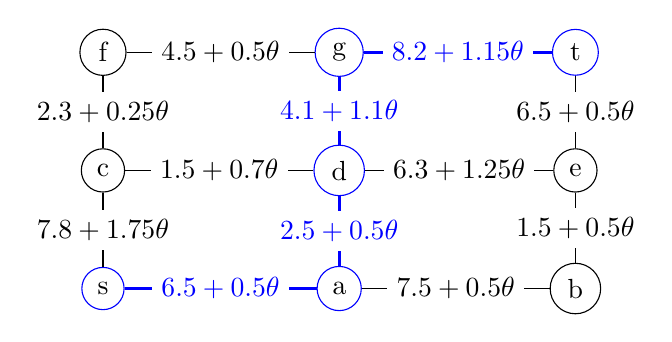
\begin{tikzpicture}
\draw
(0, 0) node[shape=circle,draw=blue] (s){s}
(3, 0) node[shape=circle,draw=blue] (a){a}
(6, 0) node[shape=circle,draw=black] (b){b}
(0, 1.5) node[shape=circle,draw=black] (c){c}
(3, 1.5) node[shape=circle,draw=blue] (d){d}
(6, 1.5) node[shape=circle,draw=black] (e){e}
(0, 3) node[shape=circle,draw=black] (f){f}
(3, 3) node[shape=circle,draw=blue] (g){g}
(6, 3) node[shape=circle,draw=blue] (t){t};     
\begin{scope}[-]
\draw[blue, very thick] (s) to node[midway, fill=white] {$6.5+0.5\theta$} (a);       
\draw (s) to node[midway, fill=white] {$7.8+1.75\theta$} (c);       
\draw (a) to node[midway, fill=white] {$7.5+0.5\theta$} (b);       
\draw[blue, very thick] (a) to node[midway, fill=white] {$2.5+0.5\theta$} (d);       
\draw (b) to node[midway, fill=white] {$1.5+0.5\theta$} (e);       
\draw (c) to node[midway, fill=white] {$1.5+0.7\theta$} (d);       
\draw (c) to node[midway, fill=white] {$2.3+0.25\theta$} (f);       
\draw (d) to node[midway, fill=white] {$6.3+1.25\theta$} (e);       
\draw[blue, very thick] (d) to node[midway, fill=white] {$4.1+1.1\theta$} (g);       
\draw (e) to node[midway, fill=white] {$6.5+0.5\theta$} (t);       
\draw (f) to node[midway, fill=white] {$4.5+0.5\theta$} (g);       
\draw[blue, very thick] (g) to node[midway, fill=white] {$8.2+1.15\theta$} (t);     
\end{scope} 
\end{tikzpicture}}
\caption{Instance of SPP-$\theta$, with in blue the optimal $s,t$-route found using Dijkstra's algorithm for the present problem, \textit{i.e.}, $\theta^0=0$.}
\label{fig:SPP_prm}
\end{center}
\vskip -0.25in
\end{figure}

We sample $\theta$ uniformly on the interval $[-1,1]$ and run CLEMO on the sampled data. In \cref{fig:SPP_prm_RLR_obj}, we show the true dependency of the optimal value of SPP-$\theta$ and $\theta$ and the prediction of CLEMO. Figure \ref{fig:SPP_prm_RLR_edges} shows the same for the dependency of three selected decision variable values. For the predictions of all decision variables, see \cref{fig:app_SPP} in the appendix. Both results show that CLEMO manages to generate locally accurate predictions. In \cref{table:SPP_loss}, we show the accuracy and the incoherence of CLEMO and the LR benchmark. %method described in Section \ref{sec:Methodology} 
 % \jannis{I think we should describe more precisely in paragraph 4.1 how this benchmark method works. How do the independent models look like? With or without complexity measure $\Omega$?} \textcolor{blue}{Daan: check, revised 4.1. We might omit the reference to methodology section then as the benchmark is described in 4.1}
We can conclude that our method finds significantly more coherent explanations without considerably conceding accuracy.


\begin{figure}[ht]
\vskip 0.2in
\begin{center}
\centerline{\subfigure[CLEMO prediction of objective value.]{\label{fig:SPP_prm_RLR_obj}\includegraphics[width=0.9\columnwidth]{./Plots/SPP_prm_RLR_obj.png}}}
\centerline{\subfigure[CLEMO prediction of a subset of decision variables.]{\label{fig:SPP_prm_RLR_edges}\includegraphics[width=0.9\columnwidth]{./Plots/SPP_prm_RLR_edges_subset.png}}}
\caption{Solution of shortest path of SPP-$\theta$ instance as determined by Dijkstra's Algorithm and as predicted by CLEMO.}
\label{fig:SPP_prm_opt}
\end{center}
\vskip -0.25in
\end{figure}


\subsection{Knapsack Problem}
Next, we present an extensive study on the Knapsack problem (KP). In this problem, we are given a set of items each with a corresponding value $v_j$ and weight $w_j$. The goal is to decide how much of each item should be chosen to maximize the total value while not exceeding the capacity, which \textit{w.l.o.g.} we set to $1$. Formulated as a linear problem this becomes $\max \{ \bm{v}^\intercal\bm{x}:\bm{w}^\intercal\bm{x}\leq 1, \bm{x}\in [0,1]^p\}$.
% \begin{equation*}\label{eqn:KP}
% \begin{array}{ll}
%   \max & \bm{v}^\intercal\bm{x}\\
%  \text{s.t.} & \bm{w}^\intercal\bm{x}\leq 1\\
%  &\bm{x}\in [0,1]^p.
% \end{array}
% \end{equation*}
We consider the parametrized KP, by setting $\bm{\theta}=(\bm{v},\bm{w})$ and use Gurobi to solve to optimality.% \jannis{which solver? and which software? Gurobi?}


This experiment compares CLEMO with two benchmark explanation methods: independently fitting the components using (i) a linear regression model (LR), and (ii) a decision tree regressor (DTR) with a maximum depth of 5, and minimum samples per leaf of 50. Here, we consider 40 instances of the KP each with $p=25$ items. The 40 instances are divided over four instance types as described by Pisinger \yrcite{pisinger_where_2005}: 1) uncorrelated, 2) weakly correlated, 3) strongly correlated, 4) inversely strongly correlated.

In \cref{table:KS_loss}, we see that compared to a linear regression approach the linear model found by CLEMO reduces the weighted incoherence 
 % \jannis{how is coherence measured? should be stated in 4.1 as well}\textcolor{blue}{Daan: $R_C$, incorporated in revised sctn 4.1} 
in the objective and the constraint by more than 50\% and 99\% respectively, while the weighted accuracy loss increased only by roughly 20\%. In \cref{fig:app_KS_type1,fig:app_KS_type2,fig:app_KS_type3,fig:app_KS_type4} in the appendix we plotted the accuracy and incoherence of each instance to strengthen our conclusion.

\begin{table}[b]
\caption{Mean weighted accuracy loss and incoherence for the KP solved optimally.}
\label{table:KS_loss}
\vskip 0.15in
\begin{center}
\begin{small}
% \begin{sc}
% \resizebox{\columnwidth}{!}{%
\begin{tabular}{cc|c|cc}
                        &        &    & \multicolumn{2}{c}{Incoherence ($R_C$)}      \\
                        & Method & Accuracy ($\ell_A$) & \multicolumn{1}{c|}{Objective} & \begin{tabular}[c]{@{}c@{}}Feasible\\ region\end{tabular} \\ \cline{2-5}
\parbox[t]{2mm}{\multirow{3}{*}{\rotatebox[origin=c]{90}{Type 1}}} & DTR    & \textbf{405}     & \multicolumn{1}{c|}{6.48} & 22.50            \\
                        & LR     & 437     & \multicolumn{1}{c|}{0.24} & 5.49          \\
                        & CLEMO & 479      & \multicolumn{1}{c|}{\textbf{0.08}} & \textbf{0.01}            \\ \cline{2-5}
\parbox[t]{2mm}{\multirow{3}{*}{\rotatebox[origin=c]{90}{Type 2}}} & DTR    & \textbf{868}      & \multicolumn{1}{c|}{20.09} & 38.55            \\
                        & LR     & 1076     & \multicolumn{1}{c|}{1.01} & 9.49            \\
                        & CLEMO &  1203      & \multicolumn{1}{c|}{\textbf{0.38}} & \textbf{0.03}           \\ \cline{2-5}
\parbox[t]{2mm}{\multirow{3}{*}{\rotatebox[origin=c]{90}{Type 3}}} & DTR    & \textbf{865}      & \multicolumn{1}{c|}{28.45} & 39.41            \\
                        & LR     & 1061      & \multicolumn{1}{c|}{1.39} & 9.90           \\
                        & CLEMO & 1189      & \multicolumn{1}{c|}{\textbf{0.58}} & \textbf{0.04}            \\ \cline{2-5}
\parbox[t]{2mm}{\multirow{3}{*}{\rotatebox[origin=c]{90}{Type 4}}} & DTR    & \textbf{893}      & \multicolumn{1}{c|}{13.80} & 37.74            \\
                        & LR     & 1111      & \multicolumn{1}{c|}{0.70} & 8.94            \\
                        & CLEMO & 1241      & \multicolumn{1}{c|}{\textbf{0.27}} & \textbf{0.03}           
\end{tabular}
% }
% \end{sc}
\end{small}
\end{center}
\vskip -0.1in
\end{table}
Besides, as datasets are randomly generated we measure the stability of explanations over resampling. For the KP, we analyze the stability of CLEMO by using 10 different randomly generated datasets, resulting in 10 surrogate models. To quantify stability we use the (normalized) standard deviation of the feature contributions of $g$ which is also used to examine the stability of LIME \cite{shankaranarayana_alime_2019}. In \cref{table:KS_stab}, we consider the (normalized) standard deviation of the contribution of the top-5 most contributing, non-zero features for each component of $h(\bm{\theta})$. Besides, we examine the feature stability index (FSI), which is based on the variables stability index as presented in \cite{visani_statistical_2022}. The FSI measures how much the order in feature contribution over the resamples on average coincides. Here, it takes values between 0 and 5, where a higher FSI indicates more stable explanations. An extensive description of the FSI can be found in section \ref{sec:KP_app} in the appendix. From \cref{table:KS_stab}, we can conclude that the stability of CLEMO is comparable to the benchmark approaches. 


\begin{table}[ht]
\caption{Mean stability measures over 10 instances per type of KP.}
\label{table:KS_stab}
\vskip 0.15in
\begin{center}
\begin{small}
% \begin{sc}
\begin{tabular}{cc|ccc}
    &        & \multicolumn{3}{c}{Stability}      \\
    & Method & \multicolumn{1}{c|}{Std.} & \multicolumn{1}{c|}{Normalized Std.}  & FSI \\ \cline{2-5}
\parbox[t]{2mm}{\multirow{3}{*}{\rotatebox[origin=c]{90}{Type 1}}} & DTR & \multicolumn{1}{c|}{0.18} & \multicolumn{1}{c|}{5.36} &2.02           \\
    & LR  & \multicolumn{1}{c|}{0.22} & \multicolumn{1}{c|}{\textbf{1.70}}&\textbf{2.44}           \\
    & CLEMO & \multicolumn{1}{c|}{\textbf{0.18}} & \multicolumn{1}{c|}{1.75} & 2.26            \\ \cline{2-5}
\parbox[t]{2mm}{\multirow{3}{*}{\rotatebox[origin=c]{90}{Type 2}}} & DTR & \multicolumn{1}{c|}{\textbf{0.14}} & \multicolumn{1}{c|}{2.74} &3.00            \\
    & LR  & \multicolumn{1}{c|}{0.19} & \multicolumn{1}{c|}{\textbf{0.74}}& \textbf{3.40}             \\
    & CLEMO & \multicolumn{1}{c|}{0.16} & \multicolumn{1}{c|}{0.81} &3.34            \\ \cline{2-5}
\parbox[t]{2mm}{\multirow{3}{*}{\rotatebox[origin=c]{90}{Type 3}}} & DTR & \multicolumn{1}{c|}{\textbf{0.14}} & \multicolumn{1}{c|}{2.77} &2.91           \\
    & LR  & \multicolumn{1}{c|}{0.20} & \multicolumn{1}{c|}{\textbf{0.71}}    &3.22         \\
    & CLEMO & \multicolumn{1}{c|}{0.16} & \multicolumn{1}{c|}{0.79}   &\textbf{3.23}       \\ \cline{2-5}
\parbox[t]{2mm}{\multirow{3}{*}{\rotatebox[origin=c]{90}{Type 4}}} & DTR & \multicolumn{1}{c|}{\textbf{0.14}} & \multicolumn{1}{c|}{2.52}  &2.99          \\
    & LR  & \multicolumn{1}{c|}{0.18} & \multicolumn{1}{c|}{\textbf{0.66}}   &3.31         \\
    & CLEMO & \multicolumn{1}{c|}{0.16} & \multicolumn{1}{c|}{0.77 }  & \textbf{3.38 }            
\end{tabular}
% \end{sc}
\end{small}
\end{center}
\vskip -0.1in
\end{table}


\begin{figure*}[h]
\vskip 0.2in
\begin{center}
  \includegraphics[width=0.82\textwidth]{./Plots/CVRP_Obj.png}
  \caption{Explanation as found by CLEMO for the objective value visualized in the present problem network structure. Also, the top 10 relative feature contributions is depicted on the right.} \label{fig:VRP_n17_obj}
    \end{center}
\vskip -0.2in
\end{figure*}

\subsection{Vehicle Routing Problem}
We consider the Capacitated Vehicle Routing problem (CVRP). An instance of this problem is given by a complete graph $G=(V,A)$ where $V$ consists of a depot node $v_0$ and $n$ client nodes each with a corresponding demand $d_j$. Moreover, each arc $(v_j,v_k)$ has associated costs $c_{jk}$. Lastly, there are $m$ vehicles, each with a capacity of $M$. The goal of the problem is to find at most $m$ routes of minimum costs such that each route starts and ends at the depot, each client is visited exactly once, and the total demand on each route does not exceed the vehicle capacity. To formulate $R_C$, we use the Miller-Tucker-Zemlin formulation for the CVRP which can be found in \cref{eqn:CVRP-app} in the appendix. The decision variables are then denoted by $x_{jk}$ and equal $1$ if arc $(v_j,v_k)$ is used in the solution and $0$ otherwise. 
% The full formulation of the problem can be found in \cref{eqn:CVRP-app} in the Appendix. 
% \jannis{we should state the name of the formulation here. Miller-Tucker-Zemlin? Also we should briefly explain why we actually need a formulation here. The reader may be confused because we are using the heuristic. Actually we should state this already in the methodology, it is a major point.}

For this experiment, we consider the parameter vector consisting of the demands $\bm{d}$ and the costs of the arcs from the clients to the depot $\bm{c_0}$, \textit{i.e.}, $\bm{\theta}=(\bm{d},\bm{c_0})$. The present problem has symmetric costs and consists of 16 clients and 4 vehicles. As a solver for this NP-hard problem, we let the Google OR-Tools heuristic search for a solution for 5 seconds \cite{ortools_routing}. We aim for explanations for the objective value, and which clients are visited before returning to the depot, \textit{i.e.}, the decision variables $x_{j0}$ for $j\in [n]_1$.

As shown in \cref{table:CVRP_loss} the explanation found by CLEMO is significantly more coherent without considerably losing in accuracy compared to the LR benchmark. We visualize the explanations found by CLEMO in \cref{fig:VRP_n17_obj}. In this figure, we first see the solution to the present problem found by Google OR-Tools in gray. Next, the feature contribution of the demands and costs are visualized via node and edge colors respectively.
% \jannis{Why are we showing the picture for the decision variable. Wouldnt the explanation for the objective value be more comprehensible for the reader?} 
Combined with an overview of the top 10 most contributing features, this shows which features are the key components influencing the objective value as found by the solver. Thus, \cref{fig:VRP_n17_obj} tells us that the objective value is mainly affected by the distance towards the nodes far from the depot. In \cref{fig:VRP_n17_x20} in the appendix, we present an additional explanation for the decision variable $x_{20}$.
 % \jannis{Mention that another graphic is in the appendix.}
\begin{table}[b]
\caption{Weighted accuracy loss and incoherence of explaining Google OR-Tools applied to the CVRP instance using the LR benchmark and using CLEMO.}
\label{table:CVRP_loss}
\vskip 0.15in
\begin{center}
\begin{small}
% \begin{sc}
% \resizebox{\columnwidth}{!}{%
\begin{tabular}{c|cc|cc}
                  & \multicolumn{2}{c|}{Accuracy ($\ell_A$)}       & \multicolumn{2}{c}{Incoherence ($R_C$)}       \\
 &
  \multicolumn{1}{c|}{\begin{tabular}[c]{@{}c@{}}Objective\\ value\end{tabular}} &
  \begin{tabular}[c]{@{}c@{}}Decision\\ vector\end{tabular} &
  \multicolumn{1}{c|}{Objective} &
  \begin{tabular}[c]{@{}c@{}}Feasible\\ region\end{tabular} \\ \hline
LR & \multicolumn{1}{c|}{\textbf{4.24}} & 1207 & \multicolumn{1}{c|}{12.35} & 802.55 \\
CLEMO & \multicolumn{1}{c|}{4.24} & \textbf{1198} & \multicolumn{1}{c|}{\textbf{11.77}} & \textbf{780.26}
\end{tabular}
% }
% \end{sc}
\end{small}
\end{center}
\vskip -0.1in
\end{table}

\section{Conclusion \& Further Research}
In this paper, we propose CLEMO, a sampling-based method that can be used to explain arbitrary exact or heuristic solution algorithms for optimization problems. Our method provides local explanations for the objective value and decision variables of mathematical optimization models. Contrary to existing methods, CLEMO enforces explanations that are coherent with the underlying model structure which enhances transparent decision-making. By applying CLEMO to various optimization problems we have shown that we can find explanations that are significantly more coherent than benchmark explanations generated using LIME without substantially compromising prediction accuracy.

This work focuses on explaining the objective value and decision variables. However, one could easily extend the concept to explanations of other components such as constraint slacks, runtime, optimality gap, etc. Another extension of our work could be to consider other types of interpretable functions such as decision trees. Lastly, CLEMO could be a useful method to explain synergies between ML and optimization models, \textit{e.g.}, in predict-then-optimize models.

% Further work can also be conducted by analyzing the effect of different sampling strategies for obtaining a training data set as well as considering other policies for handling infeasible and unbounded problem instances during sampling. Finally, CLEMO inherently makes a trade-off between local accuracy and coherence. Thus, further hyperparameter tuning could be done to examine this trade-off. \jannis{the last two sentences are more technical details. maybe mention larger research ideas as extending it to decision trees or to the predict-then-optimize setting.}

% Further research:\\
% -Discretization of parameters\\
% -Explaining other values\\
% -Handling infeasible/unbounded samples differently\\
% -Other sampling techniques\\
% - Further parameter tuning\\
% -Predict and optimize\\
% -Use structure to improve ML models mimicking OR models

% \section*{Impact Statement}
% The goal of this work is to increase transparency and trust in decisions made by mathematical optimization models. Our introduced method allows for coherent explanations of arbitrary optimization models or heuristic solution algorithms explanations leading to more transparency and trust in mathematical decision-making for all stakeholders, from those developing optimization models to those subjected to the decision made.


% \textcolor{red}{ICML description:}
% Authors are \textbf{required} to include a statement of the potential 
% broader impact of their work, including its ethical aspects and future 
% societal consequences. This statement should be in an unnumbered 
% section at the end of the paper (co-located with Acknowledgements -- 
% the two may appear in either order, but both must be before References), 
% and does not count toward the paper page limit. In many cases, where 
% the ethical impacts and expected societal implications are those that 
% are well established when advancing the field of Machine Learning, 
% substantial discussion is not required, and a simple statement such 
% as the following will suffice:

% ``This paper presents work whose goal is to advance the field of 
% Machine Learning. There are many potential societal consequences 
% of our work, none which we feel must be specifically highlighted here.''

% The above statement can be used verbatim in such cases, but we 
% encourage authors to think about whether there is content which does 
% warrant further discussion, as this statement will be apparent if the 
% paper is later flagged for ethics review.


% \section{Old}
% In this section, we present a framework for explanations for optimization models by using the principles of XAI and by resolving the aforementioned deficiencies called \textcolor{red}{Local Explanations for Mathematical Optimization with Necessitated Structure (LEMONS)}. We note our proposed method is (optimization) model-agnostic, meaning it works irrespective of the underlying structure of the underlying model. Notably, sensitivity analysis can be interchangeably used for explanation. 

% \jannis{JK: It would be nice to mention the four goals here you were listing: local accurate,... etc. Then in the following subsection we can show for each point how we achieve it.}

% Consider the following optimization problem with input parameter $x\in X\subseteq \mathbb{R}^p$ consisting of a feasibility set $Z(x)\subseteq\mathbb{R}^n$ over which is optimized and an objective function $h:Z\times X\rightarrow \mathbb{R}$ which evaluates the decision vectors $z\in Z$ \jannis{JK: I find it confusing to use $x$ for the parameters of the problem}. Formally written as
% \begin{equation}
%     \min_{z\in Z(x)}h(z,x).
% \end{equation}
% Given an additional solver $\mathcal{S}_x$ we write the optimization model as the combination $(h,Z,\mathcal{S},x)$. An optimal solution and the solution found by $\mathcal{S}$ are denoted by respectively $z^*,z^{\mathcal{S}}$. For such models different outputs of such a model that can be measured. Our method allows for explanations of all such outputs by examining how the parameters influence these aspects. Measurable components of an optimization model explained by our approach include, but are not limited to, the following \jannis{JK: We should only state the main components here for which we designed the regularizers. All the others should be mentioned in the end.}:
% \begin{table}[H]
% \begin{center}\
% \begin{tabular}{ll}
% - Objective value       & - Decision vector\\
% - Feasibility of vector & - Optimality of vector\\
% - Optimality gap        & - Dual value\\
% - Slack values          & - Constraint feasibility\\
% - Runtime               & - $\#$iterations
% \end{tabular}\
% \end{center}
% \vskip -0.15in
% \end{table}
% Given a vector of measurable aspects $y\in Y \subseteq\mathbb{R}^q$ for which we want an explanation we encode the optimization model as a target function $f(x)=y$. 

% As mentioned earlier various components of $y$ can be correlated via the underlying structure of the model. Some evident dependable relations include the link between objective value and decision vector via objective function $h$, between slack values and decision vectors via the constraint functions. We argue that for many optimization problem $h$ and constraint functions are known, e.g., problems with LP formulations. Besides, many solvers output an objective value and a decision vector. We write $l(y): \mathbb{R}^q \rightarrow \mathbb{R}^r$ such that if $l(y) = 0$ holds when the known links between the components of $y$ imposed by the underlying model hold.

% \subsection{Sampling}
% We recall that optimization models do not require model training per se. Depending on the problem at hand adequate existing optimization methods are available, from exact algorithms to heuristics. This fundamental difference with respect to ML models which require a dataset to train on calls for a strategy for our method needs to create a dataset of problem instances. Subject to the problem at hand, sampling can be done by perturbing the model's input parameters randomly, according to relevant distributions or with a set of pre-determined rules, e.g., using discretization. 
% \paragraph{Sampling strategy examples}
% \jannis{JK: Only show here the final sampling strategy which we are using.}
% Considering an optimization model given by parameter vector $x\in X$. The components of $x$ can be perturbed in different ways. For example, one can perturb each element by adding an error drawn from a normal distribution with mean zero and variance scaled to its original value, which is standard used in our method
% \begin{equation}\label{eq:nrml_prtb}
%     \hat{x}_i= x_i + e_i, \quad  e_i\sim \mathcal{N}(0,\varsigma x_i),\; \varsigma\in\mathbb{R}_{++}.
% \end{equation}
% One could also opt to perturb at most by an $\epsilon\in\mathbb{R}_{++}$, e.g., checking the effect of rounding parameters to a certain number of digits:
% \begin{equation}\label{eq:epsl_prtb}
%     \hat{x}_i= x_i + \lambda_i\epsilon, \quad \lambda_i\sim \mathcal{U}[0,1],\; \epsilon\in\mathbb{R}_{++}.
% \end{equation}
% As a last example, a user could opt to perturb relatively, e.g., checking the effect of parameters being in a $\pm 10\%$ interval:
% \begin{equation}\label{eq:sclr_prtb}
%     \hat{x}_i= \lambda_i x_i, \quad  \lambda_i\sim \mathcal{U}[b_0,b_1],\; b_0,b_1\in\mathbb{R}_{+}.
% \end{equation}

% Next, we note that ad hoc sampling could result in infeasible or unbounded instances. We provide different approaches to cope with infeasible and unbounded instances each with corresponding drawbacks:
% \textcolor{red}{DO: Only show here the final sampling strategy which we are using.}
% \begin{enumerate}
%     \item Replace unfeasible and unbounded samples with feasible bounded instances. Drawback: might not give full picture of the whole optimization model.
%     \item Ensure optimization model can handle unfeasible and unbounded instance, e.g., by assigning a fixed large or small value to the target variable for unfeasible and unbounded instances. Drawback: might lead to unrealistic fit of surrogate model resulting in poor explanations.
%     \item Categorize target variable such that unbounded and unfeasible are output categories, e.g., target variable $[\pm 0\%, \pm 10\%$], more than $10\%$ deviation, unbounded, unfeasible. Drawback: Explanations do not provide direct relation between features and target variables.
% \end{enumerate} 

% \subsection{Finding and evaluating explanations}
% Consider an optimization model encoded as a function $f$ and an instance given by input parameters $x$. We also know relations between the outputs encoded by $l\circ f: \mathbb{R}^p \rightarrow \mathbb{R}^r$. Moreover, we consider a set of samples $\mathcal{X}$. Using our method, an explanation is produced by extracting the rules, feature contributions and/or feature importances from a function $g$. To find such $g$, our method evaluates the functions in set $G$ on a combination of desirable characteristics for explainers. 
 
% First, a surrogate $g$ should be locally accurate to our original model. To do this we define locality we weigh samples that based on their proximity to $x$. The weights of the samples are given by a proximity function, e.g., the radial basis function (rbf) kernel 
% \begin{equation}
% \pi_x(\hat{x}) = \exp(-D(x,\hat{x})^2/\nu^2)\label{eq:rbf},
% \end{equation}
% where $\nu$ is the kernel parameter and $D$ is a distance function, e.g., Euclidean distance. Then, local accuracy can be measured using a weighted loss function, denoted by $\mathcal{L}(f,g,\pi_x)$ such as the wMSE.

% As we wish for an explanation $g$ should be intrepretable or of low complexity. This can be achieved by imposing $G$ to consist of white-box models only, which our method will do. Another measure for intrepretability is sparsity. We denote the $\Omega(g)$ for the number of features used by $g$, to measure complexity.

% Thirdly, we argued that explanations should be coherent with the underlying model structure. To quantify the incoherence, denoted by $\mathcal{C}(g, l, \pi_x)$ of an explanation we can measure the values of $l(g(\hat{x}))$ for $\hat{x}\in\mathcal{X}$, because by construction $l(f(\hat{x}))=0$. For example, we can take the weighted mean squared or weighted mean absolute value of $l(g(\hat{x}))$.

% Lastly, as datasets are randomly generated explanations may differ when reproduced. Therefore we measure the stability of explanations over resampling. To quantify stability we use concepts from literature. Shankaranarayana and Runje measure stability by the (normalized) standard deviation of the feature contributions found by $g$ \yrcite{shankaranarayana_alime_2019}. Additionally, Visani et al. introduce the variables stability index (VSI) and measures the mean concordance of the non-zero features of all pairs of explainable models $g$ \yrcite{visani_statistical_2022}. We generalize this by summing the mean concordance of the top $k$ contributing non-zero features of all pairs of explainable models $g$ over all $k\in\{1,\hdots,p\}$ to measure if the order of contribution of the features used by $g$.

% Our method finds a surrogate that maximizes a combination of local accuracy, intrepretability, and coherence with the underlying model structure. Afterwards we evaluate the stability of the method with the mentioned metrics. For surrogate $g$ the solution to the problem
% \begin{align}\label{eq:const_expl}
%     &\text{argmin}_{g\in\mathcal{G}}\mathcal{L}(f, g, \pi_x) +\lambda_\Omega\Omega(g)&\\
%     &s.t.\quad\quad l(g(\hat{x}))=0 &\forall \hat{x}\in \mathcal{X}\notag,
%     \end{align}
% where $\lambda_\Omega\geq 0$. Although this would enforce the explanation to have no incoherence over with the underlying model structure, we note that the problem in \cref{eq:const_expl} in general is difficult to solve. There is no convexity guarantee, the constraints might prohibit a (non-trivial) solution resulting in undesired outcomes. We therefore consider a Lagrangian relaxation with $\lambda_{\mathcal{C}}\geq 0$ to obtain the following problem
% \begin{align}\label{eq:relax_expl}
%     \text{argmin}_{g\in\mathcal{G}}&\mathcal{L}(f, g, \pi_x) +\lambda_{\Omega}\Omega(g)+\lambda_{\mathcal{C}}\mathcal{C}(g, l, \pi_x).
%     \end{align}
% By composition rules of convex functions we know that for $\mathcal{G} = \{ x^{\top}\beta + \beta_0 \mid (\beta, \beta_0\in\mathbb{R}^{p+1}\}$ the family of linear models finding $g$ is a convex problem for $\mathcal{L},\Omega,\mathcal{C}$ convex functions. 

% \jannis{JK: This part is only about measuring the stability. This should be part of the experiment section.} Lastly, as datasets are randomly generated explanations may differ when reproduced. Therefore we measure the stability of explanations over resampling. To quantify stability we use concepts from literature. Shankaranarayana and Runje measure stability by the (normalized) standard deviation of the feature contributions found by $g$ \yrcite{shankaranarayana_alime_2019}. Additionally, Visani et al. introduce the variables stability index (VSI) and measures the mean concordance of the non-zero features of all pairs of explainable models $g$ \yrcite{visani_statistical_2022}. We generalize this by summing the mean concordance of the top $k$ contributing non-zero features of all pairs of explainable models $g$ over all $k\in\{1,\hdots,p\}$ to measure if the order of contribution of the features used by $g$.


\begin{comment}
\section{Methodology}
In this section we present CLEMO, a novel method to provide coherent local explanations for multiple components of mathematical optimization problems \eqref{eqn:sampleproblem}. 

Consider a given instance of Problem \eqref{eqn:sampleproblem} which is parametrized by $\bm{\hat\theta}$ which we call \textit{present problem}. Additionally we have a solution algorithm $\mathcal A$ which we want to explain. The algorithm calculates feasible solutions for every problem instance of Problem \eqref{eqn:sampleproblem}. Note that this algorithm does not necessarily have to return an optimal solution; our method also applies for heuristic or approximation algorithms. The two components we aim to explain in this work are (i) the optimal objective value, and (ii) the values of the decision variables. The main idea of our method is to fit linear models $g_c: \Theta \to \mathbb R$ for every component $c\in \{ \text{obj}, x_1,\ldots ,x_p\}$. Here $\Theta$ is the parameter space containing all possible parameter vectors $\bm{\theta}$ for \eqref{eqn:sampleproblem}. For example the model $g_{x_i}$ ideally maps every parameter vector $\bm{\theta}$ to the corresponding solution value of variable $x_i$ which is returned by algorithm $\mathcal A$. We say the linear models are \textit{coherent} for instance $\bm{\theta}$ if 
\begin{equation}\label{eq:coherence1}
f(g_{x_1}(\bm{\theta}), \ldots , g_{x_p}(\bm{\theta}); \bm{\theta}) = g_{\text{obj}}(\bm{\theta}),
\end{equation}
and 
\begin{equation}\label{eq:coherence2}
(g_{x_1}(\bm{\theta}), \ldots , g_{x_p}(\bm{\theta}))\in \mathbb X(\bm{\theta})
\end{equation}
i.e., the predictions are aligned with the underlying problem structure.
% We aim to provide a \textit{local} explanation for an optimization problem as described in \cref{eqn:sampleproblem} by considering the parameter vector $\bm{\theta}$ as its features. Such an explanation will be given by an interpretable surrogate model that is locally accurate to the optimization model, is not too complex, and enforces coherence, i.e., the explanations of the different output components respect the underlying structure of the nominal optimization model. We will refer to this method as Coherent Local Explanations for Mathematical Optimization via Nominal Structure (C-LEMONS).
%Local Explanations for Mathematical Optimization via Nominal Structure (LEMONS).

To find coherent linear explanation models, we first generate a training data set $\mathcal{D}$ by sampling vectors $\bm{\theta^i}\in\Theta$, $i\in [N]$ which are close to $\bm{\hat\theta}$. For each sample $i\in [N]$ we apply algorithm $\mathcal A$ which returns a feasible solution $\bm{x^i}$. The corresponding objective function value is denoted as $v^i = f(\bm{x^i},\bm{\theta^i})$. We combine both results in one vector $\bm{y^i}\equiv (v^i, \bm{x^i})$ where $\bm{y^i}$ is the label of training data point~$\bm{\theta^i}$.
% We denote the training data set as
% \[ 
% \mathcal{D} = \{(\bm{\theta^i}, \bm{y^i}): i\in [N]\}. 
% \]
\textcolor{red}{TODO: Ilker: change notation of $g=..$}
We want to find models $g_c$ for every component $c$ which most accurately fit to the training data, i.e., $g_{\text{obj}}(\bm{\theta^i}) \approx v^i$, $g_{x_j}(\bm{\theta^i}) \approx \bm{x^i}_j$ for all $i\in[N]$ and $j\in [p]$. We denote by $g$ the vector of all functions $g_c$, i.e., $g=(g_{\text{obj}},g_{x_1},\ldots ,g_{x_p})$.

% It is important to note that solving an optimization problem dictates a structure on the output. To take the structure of the nominal problem into account, we also define the set of admissible output vectors for a given $\bm{\theta}_i$ with $i\in [n]$ by
% \[
% \mathbb{Y}_i = \{\bm{y}_i = (v_i, \bm{x}_i) : v_i = f(\bm{x}_i; \bm{\theta}_i), \bm{x}_i \in \mathbb{X}(\bm{\theta}_i)\}.
% \]
% Consequently, the output vectors in our dataset $\mathcal{D}$ satisfy $\bm{y}_i \in \mathbb{Y}_i$, for $i\in[N]$.

% Our next step is to fit a \textit{local} model $g$ belonging to the hypothesis set $\mathcal{G}$. Such a model would give for the input vector $\bm{\theta}_i$, the prediction $g(\bm{\theta}_i) \equiv \hat{\bm{y}}_i$. In order to select $g \in \mathcal{G}$, we define an empirical loss function and solve 

Finally, we solve the problem
\begin{equation}
\label{eqn:CLEMO}
\argmin_{g\in\mathcal{G}} ~ \sum_{i=1}^N w^i \big(\ell_A(g(\bm{\theta^i}), \bm{y^i}) + \lambda \ell_C(g(\bm{\theta^i}),\bm{y^i})\big),
\end{equation}
where $\mathcal{G}$ contains all $p+1$-dimensional vectors of linear functions,  the scalars $w^i \geq 0$ denote the sample weights, $\ell_A$ denotes the accuracy loss, and $\ell_C$ corresponds to the coherence loss which punishes predictors which do not admit the coherence conditions \eqref{eq:coherence1} and \eqref{eq:coherence2}. The hyperparameter $\lambda \geq 0$ is the penalty parameter balancing the two involved losses. 

In principal any appropriate loss function can be used for the accuracy and the coherence loss. We propose to use the squared loss
\[
\ell_A(g(\bm{\theta^i}), \bm{y^i}) = (g_{\text{obj}}(\bm{\theta^i}) - v^i)^2 + \sum_{j=1}^{p} (g_{x_j}(\bm{\theta^i}) - \bm{x^i}_j)^2
\]
as accuracy loss and for the coherence loss we use
\begin{align*}
\ell_C(g(\bm{\theta^i}), \bm{y^i}) = & (g_{\text{obj}}(\bm{\theta^i}) - f(g_{x_1}(\bm{\theta^i}), \ldots , g_{x_p}(\bm{\theta^i}))^2  \\ 
& + \delta\left( \left((g_{x_1}(\bm{\theta^i}),\ldots , g_{x_p}(\bm{\theta^i})\right), \mathbb X(\bm{\theta^i}) \right)
\end{align*}
where $\delta(\bm{x},\mathbb X(\bm{\theta}))$ denotes a distance between a point $\bm{x}$ and the feasible set $\mathbb X(\bm{\theta})$. The first term of the $\ell_C$-loss punishes the violation of the coherence condition \eqref{eq:coherence1} while the second term punishes the violation of the coherence condition \eqref{eq:coherence2}. A natural choice for the distance measure is to punish the sum of constraint violations of a solution. For example, if the feasible region is given by a set of constraints $\mathbb X(\bm{\theta^i})=\{ \bm{x}: \gamma_t(\bm{x},\bm{\theta^i}) \le 0, \ t=1,\ldots ,T\}$, then we define 
\[\delta\left(\bm{x},\mathbb X(\bm{\theta^i})\right) = \sum_{t=1}^{T} \max\{ 0, \gamma_t(\bm{x},\bm{\theta^i})\}.\] 
Note that all loss functions can depend on hyperparameters, which we examine in the experiment section.

\begin{lemma}\label{lem:convex}
    \begin{enumerate}
        \item For $g$ convex functions, and $\ell_A, \ell_C$ convex and non-decreasing in each argument, the expression in \cref{eqn:CLEMO} is convex.
        \item For $g$ affine, and $\ell_A, \ell_C$ convex functions, the expression in \cref{eqn:CLEMO} is convex.
    \end{enumerate}
\end{lemma}
\begin{example}
\textcolor{red}{JK:Actually after editing and reading everything I do not see why this example helps in understanding the concept. I think in its general version it is actually more clear. I would prefer to have a two-dimensional linear optimization example here and show how the loss function looks.}Suppose that we solve the linear optimization problems $
\min\{\bm{c}^\intercal \bm{x} : \bm{A}\bm{x} = \bm{b}, \bm{x} \geq \bm{0}\}$. Using now the formulation \eqref{eqn:sampleproblem}, we have $\bm{\theta} = (\bm{c}, \bm{A}, \bm{b})$, $f(\bm{x}; \bm{\theta}) = \bm{c}^\intercal \bm{x}$, and $\mathbb{X}(\bm{\theta}) = \{\bm{x} : \bm{A} \bm{x} = \bm{b}, \bm{x} \geq \bm{0}\}$. We then sample input $\bm{\theta}_i = (\bm{c}_i, \bm{A}_i, \bm{b}_i)$, and solve $\min\{\bm{c}_i^\intercal \bm{x} : \bm{A}_i\bm{x} = \bm{b}_i, \bm{x} \geq \bm{0}\}$ to obtain the optimal solution $\bm{x}_i$. This yields the output vector $\bm{y}_i \in \mathbb{Y}_i = \{(v_i, \bm{x}_i) : v_i = \bm{c}_i^\intercal\bm{x}_i, ~\bm{x}_i \in \mathbb{X}(\bm{\theta}_i)\}$. Now, we have the dataset $\mathcal{D}$ consisting of $(\bm{\theta}_i, \bm{y}_i)$ pairs. 

As for our local model, we restrict our hypothesis set $\mathcal{G}$ to linear models. Then, we have the predictions 
\[
\hat{\bm{y}}_i(\bm{\beta}) = (\underset{\hat v^i(\bm{\beta})}{\underbrace{\bm{\beta}_v^\intercal \bm{\theta}_i}}, \underset{\hat{\bm{x}}_i(\bm{\beta})}{\underbrace{\bm{\beta}_{x_1}^\intercal\bm{\theta}_i, \dots, \bm{\beta}_{x_p}^\intercal\bm{\theta}_i)}},
\]
where the parameter vector is $\bm{\beta} = (\bm{\beta}_v, \bm{\beta}_{x_1}, \dots, \bm{\beta}_{x_p})$.
For the functions $\ell_A$ and $\ell_C$, we use the squared error and hinge losses. This leads to the following convex optimization problem
\[
\begin{array}{llll}
\argmin_{\bm{\beta}} & \sum_{i=1}^N w^i 
\bigg(&
\|\hat{\bm{y}}_i(\bm{\beta}) - \bm{y}_i\|^2 &+ \\
&& \lambda_1(\hat{v}_i(\bm{\beta}) - \bm{c}_i^\intercal\hat{\bm{x}}_i(\bm{\beta}))^2 &+ \\
& &\lambda_2 \|\bm{A}_i\hat{\bm{x}}_i(\bm{\beta}) - \bm{b}_i\|^2 &+\\
& & \lambda_3\min\{\bm{0}, \hat{\bm{x}}_i(\bm{\beta})\}\bigg).&
\end{array}
\]
\end{example}

\begin{remark}
    CLEMO can easily be adjusted if only a subset of components $x_j$ has to be explained. In this case, we replace $g_{x_k}(\bm{\theta}^i)$ by the true value $\bm{x}^i_k$ in the above model for all components $x_k$ which do not have to be explained.
\end{remark}

\end{comment}

% \section{Electronic Submission}
% \label{submission}

% Submission to ICML 2025 will be entirely electronic, via a web site
% (not email). Information about the submission process and \LaTeX\ templates
% are available on the conference web site at:
% \begin{center}
% \textbf{\texttt{http://icml.cc/}}
% \end{center}

% The guidelines below will be enforced for initial submissions and
% camera-ready copies. Here is a brief summary:
% \begin{itemize}
% \item Submissions must be in PDF\@. 
% \item If your paper has appendices, submit the appendix together with the main body and the references \textbf{as a single file}. Reviewers will not look for appendices as a separate PDF file. So if you submit such an extra file, reviewers will very likely miss it.
% \item Page limit: The main body of the paper has to be fitted to 8 pages, excluding references and appendices; the space for the latter two is not limited in pages, but the total file size may not exceed 10MB. For the final version of the paper, authors can add one extra page to the main body.
% \item \textbf{Do not include author information or acknowledgements} in your
%     initial submission.
% \item Your paper should be in \textbf{10 point Times font}.
% \item Make sure your PDF file only uses Type-1 fonts.
% \item Place figure captions \emph{under} the figure (and omit titles from inside
%     the graphic file itself). Place table captions \emph{over} the table.
% \item References must include page numbers whenever possible and be as complete
%     as possible. Place multiple citations in chronological order.
% \item Do not alter the style template; in particular, do not compress the paper
%     format by reducing the vertical spaces.
% \item Keep your abstract brief and self-contained, one paragraph and roughly
%     4--6 sentences. Gross violations will require correction at the
%     camera-ready phase. The title should have content words capitalized.
% \end{itemize}

% \subsection{Submitting Papers}

% \textbf{Anonymous Submission:} ICML uses double-blind review: no identifying
% author information may appear on the title page or in the paper
% itself. \cref{author info} gives further details.

% \medskip

% Authors must provide their manuscripts in \textbf{PDF} format.
% Furthermore, please make sure that files contain only embedded Type-1 fonts
% (e.g.,~using the program \texttt{pdffonts} in linux or using
% File/DocumentProperties/Fonts in Acrobat). Other fonts (like Type-3)
% might come from graphics files imported into the document.

% Authors using \textbf{Word} must convert their document to PDF\@. Most
% of the latest versions of Word have the facility to do this
% automatically. Submissions will not be accepted in Word format or any
% format other than PDF\@. Really. We're not joking. Don't send Word.

% Those who use \textbf{\LaTeX} should avoid including Type-3 fonts.
% Those using \texttt{latex} and \texttt{dvips} may need the following
% two commands:

% {\footnotesize
% \begin{verbatim}
% dvips -Ppdf -tletter -G0 -o paper.ps paper.dvi
% ps2pdf paper.ps
% \end{verbatim}}
% It is a zero following the ``-G'', which tells dvips to use
% the config.pdf file. Newer \TeX\ distributions don't always need this
% option.

% Using \texttt{pdflatex} rather than \texttt{latex}, often gives better
% results. This program avoids the Type-3 font problem, and supports more
% advanced features in the \texttt{microtype} package.

% \textbf{Graphics files} should be a reasonable size, and included from
% an appropriate format. Use vector formats (.eps/.pdf) for plots,
% lossless bitmap formats (.png) for raster graphics with sharp lines, and
% jpeg for photo-like images.

% The style file uses the \texttt{hyperref} package to make clickable
% links in documents. If this causes problems for you, add
% \texttt{nohyperref} as one of the options to the \texttt{icml2025}
% usepackage statement.


% \subsection{Submitting Final Camera-Ready Copy}

% The final versions of papers accepted for publication should follow the
% same format and naming convention as initial submissions, except that
% author information (names and affiliations) should be given. See
% \cref{final author} for formatting instructions.

% The footnote, ``Preliminary work. Under review by the International
% Conference on Machine Learning (ICML). Do not distribute.'' must be
% modified to ``\textit{Proceedings of the
% $\mathit{42}^{nd}$ International Conference on Machine Learning},
% Vancouver, Canada, PMLR 267, 2025.
% Copyright 2025 by the author(s).''

% For those using the \textbf{\LaTeX} style file, this change (and others) is
% handled automatically by simply changing
% $\mathtt{\backslash usepackage\{icml2025\}}$ to
% $$\mathtt{\backslash usepackage[accepted]\{icml2025\}}$$
% Authors using \textbf{Word} must edit the
% footnote on the first page of the document themselves.

% Camera-ready copies should have the title of the paper as running head
% on each page except the first one. The running title consists of a
% single line centered above a horizontal rule which is $1$~point thick.
% The running head should be centered, bold and in $9$~point type. The
% rule should be $10$~points above the main text. For those using the
% \textbf{\LaTeX} style file, the original title is automatically set as running
% head using the \texttt{fancyhdr} package which is included in the ICML
% 2025 style file package. In case that the original title exceeds the
% size restrictions, a shorter form can be supplied by using

% \verb|\icmltitlerunning{...}|

% just before $\mathtt{\backslash begin\{document\}}$.
% Authors using \textbf{Word} must edit the header of the document themselves.

% \section{Format of the Paper}

% All submissions must follow the specified format.

% \subsection{Dimensions}




% The text of the paper should be formatted in two columns, with an
% overall width of 6.75~inches, height of 9.0~inches, and 0.25~inches
% between the columns. The left margin should be 0.75~inches and the top
% margin 1.0~inch (2.54~cm). The right and bottom margins will depend on
% whether you print on US letter or A4 paper, but all final versions
% must be produced for US letter size.
% Do not write anything on the margins.

% The paper body should be set in 10~point type with a vertical spacing
% of 11~points. Please use Times typeface throughout the text.

% \subsection{Title}

% The paper title should be set in 14~point bold type and centered
% between two horizontal rules that are 1~point thick, with 1.0~inch
% between the top rule and the top edge of the page. Capitalize the
% first letter of content words and put the rest of the title in lower
% case.

% \subsection{Author Information for Submission}
% \label{author info}

% ICML uses double-blind review, so author information must not appear. If
% you are using \LaTeX\/ and the \texttt{icml2025.sty} file, use
% \verb+\icmlauthor{...}+ to specify authors and \verb+\icmlaffiliation{...}+ to specify affiliations. (Read the TeX code used to produce this document for an example usage.) The author information
% will not be printed unless \texttt{accepted} is passed as an argument to the
% style file.
% Submissions that include the author information will not
% be reviewed.

% \subsubsection{Self-Citations}

% If you are citing published papers for which you are an author, refer
% to yourself in the third person. In particular, do not use phrases
% that reveal your identity (e.g., ``in previous work \cite{langley00}, we
% have shown \ldots'').

% Do not anonymize citations in the reference section. The only exception are manuscripts that are
% not yet published (e.g., under submission). If you choose to refer to
% such unpublished manuscripts \cite{anonymous}, anonymized copies have
% to be submitted
% as Supplementary Material via OpenReview\@. However, keep in mind that an ICML
% paper should be self contained and should contain sufficient detail
% for the reviewers to evaluate the work. In particular, reviewers are
% not required to look at the Supplementary Material when writing their
% review (they are not required to look at more than the first $8$ pages of the submitted document).

% \subsubsection{Camera-Ready Author Information}
% \label{final author}

% If a paper is accepted, a final camera-ready copy must be prepared.
% %
% For camera-ready papers, author information should start 0.3~inches below the
% bottom rule surrounding the title. The authors' names should appear in 10~point
% bold type, in a row, separated by white space, and centered. Author names should
% not be broken across lines. Unbolded superscripted numbers, starting 1, should
% be used to refer to affiliations.

% Affiliations should be numbered in the order of appearance. A single footnote
% block of text should be used to list all the affiliations. (Academic
% affiliations should list Department, University, City, State/Region, Country.
% Similarly for industrial affiliations.)

% Each distinct affiliations should be listed once. If an author has multiple
% affiliations, multiple superscripts should be placed after the name, separated
% by thin spaces. If the authors would like to highlight equal contribution by
% multiple first authors, those authors should have an asterisk placed after their
% name in superscript, and the term ``\textsuperscript{*}Equal contribution"
% should be placed in the footnote block ahead of the list of affiliations. A
% list of corresponding authors and their emails (in the format Full Name
% \textless{}email@domain.com\textgreater{}) can follow the list of affiliations.
% Ideally only one or two names should be listed.

% A sample file with author names is included in the ICML2025 style file
% package. Turn on the \texttt{[accepted]} option to the stylefile to
% see the names rendered. All of the guidelines above are implemented
% by the \LaTeX\ style file.

% \subsection{Abstract}

% The paper abstract should begin in the left column, 0.4~inches below the final
% address. The heading `Abstract' should be centered, bold, and in 11~point type.
% The abstract body should use 10~point type, with a vertical spacing of
% 11~points, and should be indented 0.25~inches more than normal on left-hand and
% right-hand margins. Insert 0.4~inches of blank space after the body. Keep your
% abstract brief and self-contained, limiting it to one paragraph and roughly 4--6
% sentences. Gross violations will require correction at the camera-ready phase.

% \subsection{Partitioning the Text}

% You should organize your paper into sections and paragraphs to help
% readers place a structure on the material and understand its
% contributions.

% \subsubsection{Sections and Subsections}

% Section headings should be numbered, flush left, and set in 11~pt bold
% type with the content words capitalized. Leave 0.25~inches of space
% before the heading and 0.15~inches after the heading.

% Similarly, subsection headings should be numbered, flush left, and set
% in 10~pt bold type with the content words capitalized. Leave
% 0.2~inches of space before the heading and 0.13~inches afterward.

% Finally, subsubsection headings should be numbered, flush left, and
% set in 10~pt small caps with the content words capitalized. Leave
% 0.18~inches of space before the heading and 0.1~inches after the
% heading.

% Please use no more than three levels of headings.

% \subsubsection{Paragraphs and Footnotes}

% Within each section or subsection, you should further partition the
% paper into paragraphs. Do not indent the first line of a given
% paragraph, but insert a blank line between succeeding ones.

% You can use footnotes\footnote{Footnotes
% should be complete sentences.} to provide readers with additional
% information about a topic without interrupting the flow of the paper.
% Indicate footnotes with a number in the text where the point is most
% relevant. Place the footnote in 9~point type at the bottom of the
% column in which it appears. Precede the first footnote in a column
% with a horizontal rule of 0.8~inches.\footnote{Multiple footnotes can
% appear in each column, in the same order as they appear in the text,
% but spread them across columns and pages if possible.}

% \begin{figure}[ht]
% \vskip 0.2in
% \begin{center}
% \centerline{\includegraphics[width=\columnwidth]{icml_numpapers}}
% \caption{Historical locations and number of accepted papers for International
% Machine Learning Conferences (ICML 1993 -- ICML 2008) and International
% Workshops on Machine Learning (ML 1988 -- ML 1992). At the time this figure was
% produced, the number of accepted papers for ICML 2008 was unknown and instead
% estimated.}
% \label{icml-historical}
% \end{center}
% \vskip -0.2in
% \end{figure}

% \subsection{Figures}

% You may want to include figures in the paper to illustrate
% your approach and results. Such artwork should be centered,
% legible, and separated from the text. Lines should be dark and at
% least 0.5~points thick for purposes of reproduction, and text should
% not appear on a gray background.

% Label all distinct components of each figure. If the figure takes the
% form of a graph, then give a name for each axis and include a legend
% that briefly describes each curve. Do not include a title inside the
% figure; instead, the caption should serve this function.

% Number figures sequentially, placing the figure number and caption
% \emph{after} the graphics, with at least 0.1~inches of space before
% the caption and 0.1~inches after it, as in
% \cref{icml-historical}. The figure caption should be set in
% 9~point type and centered unless it runs two or more lines, in which
% case it should be flush left. You may float figures to the top or
% bottom of a column, and you may set wide figures across both columns
% (use the environment \texttt{figure*} in \LaTeX). Always place
% two-column figures at the top or bottom of the page.

% \subsection{Algorithms}

% If you are using \LaTeX, please use the ``algorithm'' and ``algorithmic''
% environments to format pseudocode. These require
% the corresponding stylefiles, algorithm.sty and
% algorithmic.sty, which are supplied with this package.
% \cref{alg:example} shows an example.

% \begin{algorithm}[tb]
%    \caption{Bubble Sort}
%    \label{alg:example}
% \begin{algorithmic}
%    \STATE {\bfseries Input:} data $x_i$, size $m$
%    \REPEAT
%    \STATE Initialize $noChange = true$.
%    \FOR{$i=1$ {\bfseries to} $m-1$}
%    \IF{$x_i > x_{i+1}$}
%    \STATE Swap $x_i$ and $x_{i+1}$
%    \STATE $noChange = false$
%    \ENDIF
%    \ENDFOR
%    \UNTIL{$noChange$ is $true$}
% \end{algorithmic}
% \end{algorithm}

% \subsection{Tables}

% You may also want to include tables that summarize material. Like
% figures, these should be centered, legible, and numbered consecutively.
% However, place the title \emph{above} the table with at least
% 0.1~inches of space before the title and the same after it, as in
% \cref{sample-table}. The table title should be set in 9~point
% type and centered unless it runs two or more lines, in which case it
% should be flush left.

% % Note use of \abovespace and \belowspace to get reasonable spacing
% % above and below tabular lines.

% \begin{table}[t]
% \caption{Classification accuracies for naive Bayes and flexible
% Bayes on various data sets.}
% \label{sample-table}
% \vskip 0.15in
% \begin{center}
% \begin{small}
% \begin{sc}
% \begin{tabular}{lcccr}
% \toprule
% Data set & Naive & Flexible & Better? \\
% \midrule
% Breast    & 95.9$\pm$ 0.2& 96.7$\pm$ 0.2& $\surd$ \\
% Cleveland & 83.3$\pm$ 0.6& 80.0$\pm$ 0.6& $\times$\\
% Glass2    & 61.9$\pm$ 1.4& 83.8$\pm$ 0.7& $\surd$ \\
% Credit    & 74.8$\pm$ 0.5& 78.3$\pm$ 0.6&         \\
% Horse     & 73.3$\pm$ 0.9& 69.7$\pm$ 1.0& $\times$\\
% Meta      & 67.1$\pm$ 0.6& 76.5$\pm$ 0.5& $\surd$ \\
% Pima      & 75.1$\pm$ 0.6& 73.9$\pm$ 0.5&         \\
% Vehicle   & 44.9$\pm$ 0.6& 61.5$\pm$ 0.4& $\surd$ \\
% \bottomrule
% \end{tabular}
% \end{sc}
% \end{small}
% \end{center}
% \vskip -0.1in
% \end{table}

% Tables contain textual material, whereas figures contain graphical material.
% Specify the contents of each row and column in the table's topmost
% row. Again, you may float tables to a column's top or bottom, and set
% wide tables across both columns. Place two-column tables at the
% top or bottom of the page.

% \subsection{Theorems and such}
% The preferred way is to number definitions, propositions, lemmas, etc. consecutively, within sections, as shown below.
% \begin{definition}
% \label{def:inj}
% A function $f:X \to Y$ is injective if for any $x,y\in X$ different, $f(x)\ne f(y)$.
% \end{definition}
% Using \cref{def:inj} we immediate get the following result:
% \begin{proposition}
% If $f$ is injective mapping a set $X$ to another set $Y$, 
% the cardinality of $Y$ is at least as large as that of $X$
% \end{proposition}
% \begin{proof} 
% Left as an exercise to the reader. 
% \end{proof}
% \cref{lem:usefullemma} stated next will prove to be useful.
% \begin{lemma}
% \label{lem:usefullemma}
% For any $f:X \to Y$ and $g:Y\to Z$ injective functions, $f \circ g$ is injective.
% \end{lemma}
% \begin{theorem}
% \label{thm:bigtheorem}
% If $f:X\to Y$ is bijective, the cardinality of $X$ and $Y$ are the same.
% \end{theorem}
% An easy corollary of \cref{thm:bigtheorem} is the following:
% \begin{corollary}
% If $f:X\to Y$ is bijective, 
% the cardinality of $X$ is at least as large as that of $Y$.
% \end{corollary}
% \begin{assumption}
% The set $X$ is finite.
% \label{ass:xfinite}
% \end{assumption}
% \begin{remark}
% According to some, it is only the finite case (cf. \cref{ass:xfinite}) that is interesting.
% \end{remark}
% %restatable

% \subsection{Citations and References}

% Please use APA reference format regardless of your formatter
% or word processor. If you rely on the \LaTeX\/ bibliographic
% facility, use \texttt{natbib.sty} and \texttt{icml2025.bst}
% included in the style-file package to obtain this format.

% Citations within the text should include the authors' last names and
% year. If the authors' names are included in the sentence, place only
% the year in parentheses, for example when referencing Arthur Samuel's
% pioneering work \yrcite{Samuel59}. Otherwise place the entire
% reference in parentheses with the authors and year separated by a
% comma \cite{Samuel59}. List multiple references separated by
% semicolons \cite{kearns89,Samuel59,mitchell80}. Use the `et~al.'
% construct only for citations with three or more authors or after
% listing all authors to a publication in an earlier reference \cite{MachineLearningI}.

% Authors should cite their own work in the third person
% in the initial version of their paper submitted for blind review.
% Please refer to \cref{author info} for detailed instructions on how to
% cite your own papers.

% Use an unnumbered first-level section heading for the references, and use a
% hanging indent style, with the first line of the reference flush against the
% left margin and subsequent lines indented by 10 points. The references at the
% end of this document give examples for journal articles \cite{Samuel59},
% conference publications \cite{langley00}, book chapters \cite{Newell81}, books
% \cite{DudaHart2nd}, edited volumes \cite{MachineLearningI}, technical reports
% \cite{mitchell80}, and dissertations \cite{kearns89}.

% Alphabetize references by the surnames of the first authors, with
% single author entries preceding multiple author entries. Order
% references for the same authors by year of publication, with the
% earliest first. Make sure that each reference includes all relevant
% information (e.g., page numbers).

% Please put some effort into making references complete, presentable, and
% consistent, e.g. use the actual current name of authors.
% If using bibtex, please protect capital letters of names and
% abbreviations in titles, for example, use \{B\}ayesian or \{L\}ipschitz
% in your .bib file.

% \section*{Accessibility}
% Authors are kindly asked to make their submissions as accessible as possible for everyone including people with disabilities and sensory or neurological differences.
% Tips of how to achieve this and what to pay attention to will be provided on the conference website \url{http://icml.cc/}.

% \section*{Software and Data}

% If a paper is accepted, we strongly encourage the publication of software and data with the
% camera-ready version of the paper whenever appropriate. This can be
% done by including a URL in the camera-ready copy. However, \textbf{do not}
% include URLs that reveal your institution or identity in your
% submission for review. Instead, provide an anonymous URL or upload
% the material as ``Supplementary Material'' into the OpenReview reviewing
% system. Note that reviewers are not required to look at this material
% when writing their review.

% % Acknowledgements should only appear in the accepted version.
% \section*{Acknowledgements}

% \textbf{Do not} include acknowledgements in the initial version of
% the paper submitted for blind review.

% If a paper is accepted, the final camera-ready version can (and
% usually should) include acknowledgements.  Such acknowledgements
% should be placed at the end of the section, in an unnumbered section
% that does not count towards the paper page limit. Typically, this will 
% include thanks to reviewers who gave useful comments, to colleagues 
% who contributed to the ideas, and to funding agencies and corporate 
% sponsors that provided financial support.

% \section*{Impact Statement}

% Authors are \textbf{required} to include a statement of the potential 
% broader impact of their work, including its ethical aspects and future 
% societal consequences. This statement should be in an unnumbered 
% section at the end of the paper (co-located with Acknowledgements -- 
% the two may appear in either order, but both must be before References), 
% and does not count toward the paper page limit. In many cases, where 
% the ethical impacts and expected societal implications are those that 
% are well established when advancing the field of Machine Learning, 
% substantial discussion is not required, and a simple statement such 
% as the following will suffice:

% ``This paper presents work whose goal is to advance the field of 
% Machine Learning. There are many potential societal consequences 
% of our work, none which we feel must be specifically highlighted here.''

% The above statement can be used verbatim in such cases, but we 
% encourage authors to think about whether there is content which does 
% warrant further discussion, as this statement will be apparent if the 
% paper is later flagged for ethics review.


% In the unusual situation where you want a paper to appear in the
% references without citing it in the main text, use \nocite
% \nocite{langley00}

\bibliography{./references_new}
\bibliographystyle{icml2025}


%%%%%%%%%%%%%%%%%%%%%%%%%%%%%%%%%%%%%%%%%%%%%%%%%%%%%%%%%%%%%%%%%%%%%%%%%%%%%%%
%%%%%%%%%%%%%%%%%%%%%%%%%%%%%%%%%%%%%%%%%%%%%%%%%%%%%%%%%%%%%%%%%%%%%%%%%%%%%%%
% APPENDIX
%%%%%%%%%%%%%%%%%%%%%%%%%%%%%%%%%%%%%%%%%%%%%%%%%%%%%%%%%%%%%%%%%%%%%%%%%%%%%%%
%%%%%%%%%%%%%%%%%%%%%%%%%%%%%%%%%%%%%%%%%%%%%%%%%%%%%%%%%%%%%%%%%%%%%%%%%%%%%%%
\newpage
\appendix
\onecolumn
\section{Appendix}
\label{sec:app}
\subsection{Mathematical Models of The Optimization Problems}
In this section, we present the formulation of the Shortest Path problem \eqref{eqn:SPP-theta-app} and the Capacitated Vehicle Routing problem \eqref{eqn:CVRP-app}. For the latter, we use the Miller-Tucker-Zemlin formulation as described by Kara et al. \yrcite{kara_note_2004}.
\paragraph{Shortest Path Problem}
\begin{align}\label{eqn:SPP-theta-app}
 \min &  \ (\bm{c}+\theta \bm{\tilde{c}})^\intercal\bm{x}&\\
 \text{s.t.} & \sum_{(s,j)\in E} x_{s,j} -  \sum_{(j,s)\in E} x_{j,s}=1&\notag\\
  & \sum_{(j,t)\in E} x_{j,t} -  \sum_{(t,j)\in E} x_{t,j}=1&\notag\\
 & \sum_{(j,k)\in E} x_{j,k} -  \sum_{(k,l)\in E} x_{k,l}=0 & \forall k \neq s,t\notag\\
& x_{e}\in\{0,1\}& \forall e\in E \notag
\end{align}
\paragraph{Capacitated Vehicle Routing Problem}
\begin{align}\label{eqn:CVRP-app}
 \min &  \ \sum_{j=0}^n\sum_{k=0,k\neq j}^n c_{jk}x_{jk}&\\
 \text{s.t.} & \sum_{k=1}^n x_{1k} \leq m&\notag\\
  & \sum_{j=1}^n x_{j1} \leq m&\notag\\
 & \sum_{k=1}^n x_{1k} \geq 1&\notag\\
 & \sum_{j=1}^n x_{j1} \geq 1&\notag\\
  & \sum_{k=0, k\neq j}^n x_{jk}=1 &j\in[n]_1\notag\\
   &\sum_{j=0, j\neq k}^n x_{jk}=1 &k\in[n]_1\notag\\
   &u_j-u_j+Mx_{jk}\leq M-d_k &j,k \in[n]_1,\quad j\neq k\notag\\
   &d_j\leq u_j\leq M &j\in[n]_1\notag\\
& x_{jk}\in\{0,1\} &j,k\in[n]_0,\quad j\neq k\notag
\end{align}

\subsection{Detailed Algorithm}
Here, we present an extensive description of our explanation method CLEMO as used in the experiments. It consists of two parts, (i) creating a training dataset (\cref{alg:CLEMO_dataset}), and (ii) finding a surrogate model (\cref{alg:CLEMO_surr}).
\begin{algorithm}[H]
   \caption{CLEMO - Creating a dataset}
   \label{alg:CLEMO_dataset}
\begin{algorithmic}
   \STATE {\bfseries Input:} Optimization problem with parameter $\bm{\theta}^0$ and solver algorithm $h$
   \STATE Initialize samples $=\{\bm{\theta}^0\}$, targets $=\{(f(\bm{x}^0;\bm{\theta}^0), \bm{x}^0)\}$, weights $=\emptyset$, distances $=\{0\}$
   \WHILE{\#samples $<1000$}
   \STATE $\bm{\theta}^i \sim \mathcal{N}(\bm{\theta}^0, 0.2\bm{\theta}^0)$
   \IF{Optimization model is feasible and bounded for $\bm{\theta}^i$}
   \STATE samples $\leftarrow$ samples $\cup\{\bm{\theta}^i\}$
   \STATE $(f(\bm{x}^i;\bm{\theta}^i),\bm{x}^i)\leftarrow h$ applied to $\bm{\theta}^i$-problem
   \STATE targets $\leftarrow$ targets $\cup\{(f(\bm{x}^i;\bm{\theta}^i),\bm{x}^i)\}$
   \STATE distances $\leftarrow$ distances $\cup\{\textsl{Euclidean distance}(\bm{\theta}^0,\bm{\theta}^i)\}$
   \ENDIF
   \ENDWHILE
   \STATE $\overline{d}=\leftarrow$ \textsl{average}(distances)
   \FOR{$\bm{\theta}^i$ in samples}
   \STATE weights $\leftarrow$ weights $\cup\{\textsl{rbf}(\bm{\theta}^0, \bm{\theta}^i, \overline{d})\}$
   \ENDFOR
   \STATE {\bfseries Return:} $\mathcal{D}$ $\leftarrow$ (samples, targets, weights)
\end{algorithmic}
\end{algorithm}

\begin{algorithm}[H]
   \caption{CLEMO - Finding surrogate model}
   \label{alg:CLEMO_surr}
\begin{algorithmic}
   \STATE {\bfseries Input:} Optimization problem, dataset $\mathcal{D}$, loss function consisting of components $\{\ell_{A_1},\ell_{A_2},R_{C_1},R_{C_2}\}$
   \FOR{output component $c\in\{f,x_1,\dots,x_p\}$ }
    \IF{$h(\bm{\theta})_c$ is a binary value}
    \STATE $(\bm{\beta}_{BM})_c\leftarrow$ \textsl{Logistic Regression fit}(samples, $h(\bm{\theta})_c$, weights)
    \ELSE
    \STATE $(\bm{\beta}_{BM})_c\leftarrow$ \textsl{Linear Regression fit}(samples, $h(\bm{\theta})_c$, weights)
    \ENDIF
   \ENDFOR
   \STATE $\mathcal{L}_j \leftarrow \{\textsl{loss}_j(\bm{\beta}_{BM}, \mathcal{D}) \mid \text{for }\textsl{loss}_j\in \{\ell_{A_1},\ell_{A_2},R_{C_1},R_{C_2}\}\}$
   \STATE $\mathcal{L}_{\max}\leftarrow$ \textsl{maximum}($\mathcal{L}_{A_1},\mathcal{L}_{A_2},\mathcal{L}_{C_1},\mathcal{L}_{C_2}$)
   \FOR{loss function component index $j$ in $\{A_1, A_2, C_1, C_2\}$}
   \IF{$\mathcal{L}_j \in\{ \mathcal{L}_{\max},0\}$}
   \STATE $\lambda_j\leftarrow 1$
   \ELSE
   \STATE $\lambda_j\leftarrow 0.5\mathcal{L}_{\max}/\mathcal{L}_j$
   \ENDIF
   \ENDFOR
   \STATE \textsl{total\_loss\_function} $\leftarrow \lambda_{A_1}\ell_{A_1} + \lambda_{A_2}\ell_{A_2}+ \lambda_{C_1}R_{C_1} +  \lambda_{C_2}R_{C_2}$
\STATE $\bm{\beta}_{CL}\leftarrow \textsl{argmin}_{\bm{\beta}}\:\textsl{total\_loss\_function}(\bm{\beta}, \mathcal{D})$ using $\bm{\beta}_{BM}$ as a warm start
   \STATE {\bfseries Return:} Interpretable function $\bm{\beta}_{CL}$
\end{algorithmic}
\end{algorithm}

\subsection{Coherence for Linear Optimization Problems}
\label{sec:app3}

In this section we prove the statement that independent fitting of linear predictors leads to objective coherence under certain assumptions. 

\begin{theorem}\label{thm:provably_coherent}
The minimizers of the weighted least-square problems
\[
\min_{\bm{\beta}_{f}} \ \sum_{i=0}^{N} w^i\| f(\bm{x}^i;\bm{\theta}^i) - \bm{\beta}_{f}^\intercal\bm{\theta}^i \|^2 \]
and 
\[
\min_{\bm{\beta}_{x_j}} \ \sum_{i=0}^{N} w^i\| \bm{x}^i_j - \bm{\beta}_{x_j}^\intercal\bm{\theta}^i \|^2 \quad j=1,\ldots ,p .
\]
fulfill the coherence Condition \eqref{eq:coherence1}.
\end{theorem}
\begin{proof}
Since the objective function $\bm{\hat c}^\intercal \bm{x}$ is fixed and linear we have
\[
f(\bm{x}^i;\bm{\theta}^i) = \sum_{j=1}^{p} \hat c_j \bm{x}^i_j.
\]
The weighted least-squares problem has the unique optimal solution
\[
\bm{\beta}_{x_j}^* = (\bm{\Theta}^\intercal \bm{W}\bm{\Theta})^{-1} \bm{\Theta}^\intercal \bm{W} \bm{y^j} \quad j=1,\ldots ,p
\]
and 
\[
\bm{\beta}_{f}^* = (\bm{\Theta}^\intercal \bm{W}\bm{\Theta})^{-1} \bm{\Theta}^\intercal \bm{W} \bm{y^f}
\]
where $\bm{\Theta}$ is the matrix whose $i$-th row is the vector $\bm{\theta}^i$, $\bm{W}$ is the matrix with weight $w^i$ on the diagonal and zeroes elsewhere, $\bm{y^j}$ is the vector where the $i$-th entry is the value $x_j^i$ and $\bm{y^f}$ is the vector where the $i$-th entry is the value $f(\bm{x}^i;\bm{\theta}^i)$. We assume here that $(\bm{\Theta}^\intercal \bm{W}\bm{\Theta})$ is invertible. Then for any new parameter vector $\bm{\theta}$ the predicted optimal value of our model is
\begin{align*}
\bm{\theta}^\intercal\bm{\beta}_{f} & = \bm{\theta}^\intercal (\bm{\Theta}^\intercal \bm{W}\bm{\Theta})^{-1} \bm{\Theta}^\intercal \bm{W} \bm{y^f}  \\
& = \bm{\theta}^\intercal (\bm{\Theta}^\intercal \bm{W} \bm{\Theta})^{-1} \bm{\Theta}^\intercal \bm{W} \left( \sum_{j=1}^{p} \hat c_j \bm{y^{j}}\right) \\
& = \sum_{j=1}^{p} \hat c_j \bm{\theta}^\intercal (\bm{\Theta}^\intercal \bm{W}\bm{\Theta})^{-1} \bm{\Theta}^\intercal \bm{W} \bm{y^{j}} \\
& = \sum_{j=1}^{p} \hat c_j \bm{\theta}^\intercal\bm{\beta}_{x_j}
\end{align*}
which means that the predictors are coherent regarding condition \eqref{eq:coherence1}. 
\end{proof}


\subsection{Additional Experiments}
\subsubsection{Shortest Path Problem}
% \jannis{everything we show in the appendix should at some points be referred to in the main text.} 
For the SPP-$\theta$ considered in the experiments, we additionally present the prediction found by CLEMO for the decision vector compared to the values found by Dijkstra's Algorithm in \cref{fig:app_SPP}. In concordance with the results presented in the experiment section, we see CLEMO approximates the actual values relatively well.
\begin{figure}[H]
\vskip 0.2in
\begin{center}
\centerline{\includegraphics[width=0.98\columnwidth]{./Plots/Appendix/SPP_prm_RLR_edges.png}}
\caption{Decision variables solution of shortest path of SPP-$\theta$ instance as determined by Dijkstra's Algorithm and as predicted by CLEMO.}
\label{fig:app_SPP}
\end{center}
\vskip -0.2in
\end{figure}


\subsubsection{Knapsack Problem}\label{sec:KP_app}
For the knapsack problem, we applied our method on 10 instances of each of the 4 types of problems we considered. For each instance and for each method we used 10 different datasets to compare our CLEMO with benchmark methods linear regression (LR) and decision tree regressor (DTR). In \cref{fig:app_KS_type1,fig:app_KS_type2,fig:app_KS_type3,fig:app_KS_type4} we present scatter plots of the total accuracy loss and total incoherence (both conditions \eqref{eq:coherence1} and \eqref{eq:coherence2}) per instance and type of knapsack problem. Similar to the results presented in the experiment section, we find that CLEMO significantly reduces incoherence while the accuracy is compromised relatively less.

Next to the standard deviation of feature contribution, we consider an additional measure for stability, the feature stability index (FSI). This is an adaptation of the variables stability index (VSI) as presented in \cite{visani_statistical_2022}. The higher this measure, the more the non-zero features found by the different models due to resampling overlap. For a consistent explanation, the overlap should be large. As we apply CLEMO on 10 different datasets for each instance of each type of knapsack problem, we obtain 10 surrogate models given by $\bm{\beta}^1_{CL},\dots, \bm{\beta}^{10}_{CL}$. We denote $\mathcal{F}_{k,j}^i$ for the set of the top-$k$ most contributing, non-zero features of the $j$-th component of $\bm{\beta}^i_{CL}$. We define the $(k,j)$-\textsl{concordance} of two models $\bm{\beta}^{i_1}$ and $\bm{\beta}^{i_2}$ as the size of the intersection between $\mathcal{F}_{k,j}^{i_1}$ and $\mathcal{F}_{k,j}^{i_2}$ divided by the maximum potential overlap, \textit{i.e.},
\[ (k,j)\textsl{-concordance}(i_1,i_2)=\mathcal{F}_{k,j}^{i_1}\cap \mathcal{F}_{k,j}^{i_2}/ k.
\]
Let us consider the $k$-feature stability index ($k$-FSI), which is the average $(k,j)\text{-concordance}$ over all pairs $\bm{\beta}^1_{CL},\hdots \bm{\beta}^{10}_{CL}$ and all components $j$. Similar to VSI, $k$-FSI is bounded by 1 and the higher this measure $k$-FSI, the more the different models agree on the top-$k$ non-zero features of the different components and hence the more stable the method is. Lastly, we define the FSI as the sum over $k$-FSI for $k=1,\hdots 5$ resulting in a stability measure bounded by 5. When examining the FSI for CLEMO and the benchmark methods in \cref{table:KS_stab}, we conclude that CLEMO has stability similar to the general linear regression approach. 


\begin{figure}[h!]
\vskip 0.2in
\begin{center}
\centerline{\includegraphics[width=0.9\columnwidth]{./Plots/Appendix/KS_type1.png}}
\caption{Scatter plot of the total incoherence (\textit{i.e.}, coherence loss) and total accuracy losses as found by the different methods on 10 distinct sample sets per instance of the knapsack problem of type 1.}
\label{fig:app_KS_type1}
\end{center}
\vskip -0.2in
\end{figure}

\begin{figure}[h!]
\vskip 0.2in
\begin{center}
\centerline{\includegraphics[width=0.9\columnwidth]{./Plots/Appendix/KS_type2.png}}
\caption{Scatter plot of the total incoherence (\textit{i.e.}, coherence loss) and total accuracy losses as found by the different methods on 10 distinct sample sets per instance of the knapsack problem of type 2.}
\label{fig:app_KS_type2}
\end{center}
\vskip -0.2in
\end{figure}

\begin{figure}[h!]
\vskip 0.2in
\begin{center}
\centerline{\includegraphics[width=0.9\columnwidth]{./Plots/Appendix/KS_type3.png}}
\caption{Scatter plot of the total incoherence (\textit{i.e.}, coherence loss) and total accuracy losses as found by the different methods on 10 distinct sample sets per instance of the knapsack problem of type 3.}
\label{fig:app_KS_type3}
\end{center}
\vskip -0.2in
\end{figure}

\begin{figure}[h!]
\vskip 0.2in
\begin{center}
\centerline{\includegraphics[width=0.9\columnwidth]{./Plots/Appendix/KS_type4.png}}
\caption{Scatter plot of the total incoherence (\textit{i.e.}, coherence loss) and total accuracy losses as found by the different methods on 10 distinct sample sets per instance of the knapsack problem of type 4.}
\label{fig:app_KS_type4}
\end{center}
\end{figure}
\clearpage


\subsubsection{Vehicle Routing Problem}
Similar to \cref{fig:VRP_n17_obj} as presented in \cref{sec:Experiments}, we display an additional explanation for the CVRP instance solved by Google OR-Tools. In \cref{fig:VRP_n17_x20}, we see the explanation found by CLEMO for the decision variable $x_{20}$ of the considered CVRP instance solved by Google OR-Tools. From this figure, a stakeholder can deduce that arc $(2,0)$ is less likely used by Google OR-Tools when $c_{02}$ increases, but more likely when $c_{08}$ increases.
\begin{figure*}[h!]
\vskip 0.2in
\begin{center}
  \includegraphics[width=0.9\textwidth]{./Plots/CVRP_x20.png}
  \caption{Explanation as found by CLEMO for the decision variable $x_{20}$ visualized in the present problem network structure. Also, the top 10 relative feature contributions is depicted on the right.}
  \label{fig:VRP_n17_x20}
  \end{center}
\vskip -0.2in
\end{figure*}



%%%%%%%%%%%%%%%%%%%%%%%%%%%%%%%%%%%%%%%%%%%%%%%%%%%%%%%%%%%%%%%%%%%%%%%%%%%%%%%
%%%%%%%%%%%%%%%%%%%%%%%%%%%%%%%%%%%%%%%%%%%%%%%%%%%%%%%%%%%%%%%%%%%%%%%%%%%%%%%


\end{document}


% This document was modified from the file originally made available by
% Pat Langley and Andrea Danyluk for ICML-2K. This version was created
% by Iain Murray in 2018, and modified by Alexandre Bouchard in
% 2019 and 2021 and by Csaba Szepesvari, Gang Niu and Sivan Sabato in 2022.
% Modified again in 2023 and 2024 by Sivan Sabato and Jonathan Scarlett.
% Previous contributors include Dan Roy, Lise Getoor and Tobias
% Scheffer, which was slightly modified from the 2010 version by
% Thorsten Joachims & Johannes Fuernkranz, slightly modified from the
% 2009 version by Kiri Wagstaff and Sam Roweis's 2008 version, which is
% slightly modified from Prasad Tadepalli's 2007 version which is a
% lightly changed version of the previous year's version by Andrew
% Moore, which was in turn edited from those of Kristian Kersting and
% Codrina Lauth. Alex Smola contributed to the algorithmic style files.
